%% FILE: loc-diff-terms-ijac.tex
%% AUTHOR: William DeMeo, Ralph Freese
%% DATE: 1 Dec 2016
%% COPYRIGHT: (C) 2016 William DeMeo 

%%%%%%%%%%%%%%%%%%%%%%%%%%%%%%%%%%%%%%%%%%%%%%%%%%%%%%%%%%
%%                         BIBLIOGRAPHY FILE            %%
%%%%%%%%%%%%%%%%%%%%%%%%%%%%%%%%%%%%%%%%%%%%%%%%%%%%%%%%%%
%% The `filecontents` command will crete a file in the inputs directory called 
%% refs.bib containing the references in the document, in case this file does 
%% not exist already.
%% If you want to add a BibTeX entry, please don't add it directly to the
%% refs.bib file.  Instead, add it in this file between the
%% \begin{filecontents*}{refs.bib} and \end{filecontents*} lines
%% then delete the existing refs.bib file so it will be automatically generated 
%% again with your new entry the next time you run pdfaltex.
\begin{filecontents*}{refs.bib}
@book {Rose:1978,
    AUTHOR = {Rose, John S.},
     TITLE = {A course on group theory},
      NOTE = {Reprint of the 1978 original [Cambridge University Press;  MR0498810 (58
              \#16847)]},
 PUBLISHER = {Dover Publications Inc.},
   ADDRESS = {New York},
      YEAR = {1994},
     PAGES = {x+310},
      ISBN = {0-486-68194-7},
   MRCLASS = {20-01},
  MRNUMBER = {1298629},
}
@MISC {MO63675,    
    TITLE = {What groups have a second maximal subgroup below exactly four maximal subgroups?},    
    AUTHOR = {William DeMeo},
    HOWPUBLISHED = {MathOverflow},    
    NOTE = {URL: \url{http://mathoverflow.net/questions/63675} (version: 2011-05-02)},    
    EPRINT = {http://mathoverflow.net/questions/63675},    
    URL = {http://mathoverflow.net/questions/63675},    
}
@COMMENT (mathoverflow.net/users/9124)},    
@MISC {MO62495,    
    TITLE = {Which finite nonabelian groups have long chains of subgroups as intervals in their subgroup lattice?},    
    AUTHOR = {William DeMeo (mathoverflow.net/users/9124)},    
    HOWPUBLISHED = {MathOverflow},    
    NOTE = {URL: \url{http://mathoverflow.net/questions/62495} (version: 2011-04-21)},    
    EPRINT = {http://mathoverflow.net/questions/62495},    
    URL = {http://mathoverflow.net/questions/62495},    
}
@book {Suzuki:1982,
    AUTHOR = {Suzuki, Michio},
     TITLE = {Group theory. {I}},
    SERIES = {Grundlehren der Mathematischen Wissenschaften [Fundamental
              Principles of Mathematical Sciences]},
    VOLUME = {247},
      NOTE = {Translated from the Japanese by the author},
 PUBLISHER = {Springer-Verlag},
   ADDRESS = {Berlin},
      YEAR = {1982},
     PAGES = {xiv+434},
      ISBN = {3-540-10915-3},
   MRCLASS = {20-01},
  MRNUMBER = {648772 (82k:20001c)},
MRREVIEWER = {B. Chang},
}
@Book{Hungerford:1974,
  author =       {Thomas W.~Hungerford},
  title =        {Algebra},
  year =         {1974},
  publisher =    {Springer-Verlag},
  address =      {New York}
}
@book {Dixon:1996,
    AUTHOR = {Dixon, John D. and Mortimer, Brian},
     TITLE = {Permutation groups},
    SERIES = {Graduate Texts in Mathematics},
    VOLUME = {163},
 PUBLISHER = {Springer-Verlag},
   ADDRESS = {New York},
      YEAR = {1996},
     PAGES = {xii+346},
      ISBN = {0-387-94599-7},
   MRCLASS = {20B05 (20-01 20B07)},
  MRNUMBER = {1409812 (98m:20003)},
MRREVIEWER = {Martin W. Liebeck},
}
\end{filecontents*}
%:biblio
%%%%%%%%%%%%%%%%%%%%%%%%%%%%%%%%%%%%%%%%%%%%%%%%%%%%%%%%%%%%%%%%%%%%%%%%%%%%%%%%%%%%
%%                                     PREAMBLE                                   %%
%%%%%%%%%%%%%%%%%%%%%%%%%%%%%%%%%%%%%%%%%%%%%%%%%%%%%%%%%%%%%%%%%%%%%%%%%%%%%%%%%%%%
\documentclass[leqno,twoside]{article}
\headsep 0.5cm \pagestyle{myheadings}
\usepackage{amssymb,amsmath,latexsym, amsthm,enumerate, nsjom, amsfonts}
\title{}\author{}\date{}
\markboth{W.~DeMeo}{Facts on Finite Groups}\setcounter{page}{1}
%% \usepackage[dvipdfm, pdfstartview=FitH]{hyperref} % Use LaTeX and then DVI2PDF,
% or, if you plan to use packages only compatible with PDFLaTeX
\usepackage[pdftex, pdfstartview=FitH]{hyperref}

%% \usepackage{graphicx}
% Use this package if you plan to put some pictures

%% \usepackage{pinlabel}  %%% was the recommended graphics+labelling package for JLA

%If you want equations number as (2.1), where, 2 is the section number then use
\numberwithin{equation}{section} %You may omit this line if you want numbering as (1)

 \newtheorem{thm}{Theorem}[section]
 \newtheorem*{theorem}{Theorem}        % theorem environment without numbering
 \newtheorem{cor}[thm]{Corollary}
 \newtheorem*{corollary}{Corollary}     % Corollary environment without numbering 
 \newtheorem{lem}[thm]{Lemma}
 \newtheorem*{lemma}{Lemma}            % Lemma environment without numbering 
 \newtheorem*{zlem}{Zorn's Lemma}      % A special unnumbered lemma.
 \newtheorem*{monotonicity}{Monotonicity of the Commutator} % A special unnumbered lemma.
 \newtheorem{prop}[thm]{Proposition}

 \theoremstyle{definition}
 \newtheorem{defn}[thm]{Definition}
 \newtheorem{prob}{Problem}    
 \newtheorem{ex}[thm]{Example}

 \theoremstyle{remark}
 \newtheorem{rem}[thm]{Remark}
 \newtheorem{Fact}{Fact}[section]
 \newtheorem{remarks}{Remarks}



 \usepackage[paperwidth=165mm, paperheight=235mm, twoside, hmargin={25mm,20mm}, vmargin={20mm,20mm} ]{geometry}

% You may use some variations of this environments, for instance, with separate global counters
% \newtheorem{defn}{Definition}
% Also, you may use your own names for environments like
% \newtheorem{df}{Definition}
% or whatever you prefer, but, please, use them

 %%%%%%%%%%%%%%%%%%%%%%%%%%%%%%%%%%%%%%%%%%%%%%%%%%%%%%%%%%%%%%%%%
 %%% MY STUFF
 \usepackage{macros}
 \usepackage{comment}
 %%%%%%%%%%%%%%%%%%%%%%%%%%%%%%%%%%%%%%%%%%%%%%%
 %% showkeys: just comment out in the final version
 \usepackage[notref,notcite]{showkeys}
 %%%%%%%%%%%%%%%%%%%%%%%%%%%%%%%%%%%%%%%%%%%%%%%
 %% removed these for jla
 % \usepackage{amsmath,amssymb,amsthm} %, amsmath are included by default}
 %% \usepackage{amscd}
 \usepackage{mathtools}
 % \usepackage{scrextend}
 \usepackage{lmodern}% http://ctan.org/pkg/lm
 %\usepackage{bm}
 \usepackage{latexsym,enumerate,scalefnt,ifthen} %,mathrsfs,
 \usepackage{stmaryrd}
 \SetSymbolFont{stmry}{bold}{U}{stmry}{m}{n}
 \usepackage[mathscr]{euscript}
 %% \usepackage[colorlinks=true,urlcolor=black,linkcolor=black,citecolor=black]{hyperref}
 \usepackage{scalefnt}
 \usepackage{tikz}
 \usepackage{color}
 %% \usepackage[margin=1.5in]{geometry}

 \newboolean{todos}
 \setboolean{todos}{true}  % set to true to include TODO statements
 %   \setboolean{todos}{false}  % set to false to exclude TODO statements

   %%% INTENDED USE OF THE arxiv AND extralong BOOLEAN VARIABLES
   %%% -- The brief journal version should have `arxiv` and `extralong` variables set to false.
   %%% -- The arxiv version should have `arxiv` set to true and `extralong` set to false.
   %%% -- The extralong version may contain notes intended for our own personal reference.
   %%%    For the extralong version, set both `arxiv` and `extralong` to true.   
   \newboolean{arxiv}
   \setboolean{arxiv}{true}  % set to true to include almost everything
   \setboolean{arxiv}{false}  % set to false for the brief version

   \newboolean{extralong}
   \setboolean{extralong}{true}  % set to true to include everything
   %% \setboolean{extralong}{false}  % set to false for the long (but not too long) version

   \newboolean{footnotes}
   \setboolean{footnotes}{true}  % set to true to include footnotes
   \setboolean{footnotes}{false}  % set to false for no footnotes


   \newboolean{draftsecskip}
   \setboolean{draftsecskip}{true}
   % \setboolean{draftsecskip}{false}

   \newboolean{thetanotation}
   \setboolean{thetanotation}{true}
   \setboolean{thetanotation}{false}


   % \newcommand\draftsecskip{\ifthenelse{\boolean{draftsecskip}}{\medskip}{}}
   \newcommand\draftsecskip{\ifthenelse{\boolean{draftsecskip}}{\newpage}{}}

   %%%% wjd: adding pagebreaks for ``draft mode'' to reduce printing costs
   %%%%      To turn off these unnecessary page breaks, set `draft` to false:
   \newboolean{draft}
   \setboolean{draft}{true}  % set to true to include footnotes

   
%%%%%%%%%%%%%%%%%%%%%%%%%%%%%%%%%% End of user-defined macros %%%


\begin{document}
\thispagestyle{empty}

% \begin{flushleft}
% \vspace*{-1.1cm} {\sc  Novi Sad J.\ Math.}\\ {\sc Vol.\ XX, No.\ Y, 20ZZ, ??-??}
% \end{flushleft}
\begin{flushright}
\vspace*{-1.1cm} {{\small \sffamily Last updated: 17 March 2017}}
\end{flushright}
\vspace{0.8cm}
% PRAVLJENJE NASLOVA
\begin{center}
  {\large \bf FACTS ON FINITE GROUPS: a smorgasbord of known facts, experimental data and other trivia
    %\footnote{This is one place where you can put acknowledgement}
} \vspace*{3mm}

% Title should be in upper case

{\bf William DeMeo\footnote{Department of Mathematics, University of Hawaii,\\
    e-mail: \href{mailto:williamdemeo@gmail.com}{williamdemeo@gmail.com}}}
\end{center}
% Authors should be ordered alphabetically
% Please, use your full name and put an email address in affiliation. The example with underline in e-mail address:
%\href{mailto:my_address@wikibooks.org}{my\_address@wikibooks.org}

\begin{abstract}
  We present here a rough and unpolished collection of potentially useful facts
  about finite groups, most (if not all) of which are well known. Much of this information
  appeared in disparate notes from research seminars, and the author received requests
  to collect this information and post it somewhere for reference and so that it may be easily
  cited in other works.  With this purpose in mind, the proper BibTeX data are displayed on the
  last page below.
\end{abstract}

%%%%%%%%%%%%%%%%%%%%   Start of main body of article


\section{Examples of Cayley's Theorem on Permutation Representations of Finite Groups}
\label{sec:introduction}
Let $X$ be a finite set and consider the set $X^X$ of all maps from $X$ to
itself, which, when endowed with composition of maps and the identity mapping,
forms a monoid, $\<X^X; \circ, \id{X}\>$.  The submonoid $S_X$ of all bijective
maps in $X^X$ is a group, the \emph{symmetric group on $X$}.  When the
underlying set isn't important, we write $S_n$ to denote the generic
symmetric group on an $n$-element set. 

If we have defined some set $F$ of basic operations on $X$, so that
$\bX = \<X; F\>$ is an algebra, then two other important submonoids of
$X^X$ are $\End(\bX)$, the set of maps in $X^X$ which respect all 
operations in $F$, and $\Aut(\bX)$, the set of bijective maps in  $X^X$ which
respect all operations in $F$.  It is apparent from the definition that
 $\Aut(\bX)= S_X \cap \End(\bX)$, and  $\Aut(\bX)$ is a submonoid of $\End(\bX)$
 and a subgroup of $S_X$.  These four fundamental monoids
 associated with the algebra $\bX$ are shown in the diagram below. 

\begin{center}
  \begin{tikzpicture}[scale=.7]
%    \node (Aut) at (0,0) [fill,circle,inner sep=1pt] {};
    \draw[font=\small] (0,0) node {$\Aut(\bX)$};
%    \node (End) at (-2,2) [fill,circle,inner sep=1pt] {};
    \draw[font=\small] (-2,2) node {$\End(\bX)$};
%    \node (Sx) at (2,2) [fill,circle,inner sep=1pt] {};
%    \draw[font=\small] (2,2) node {$S_X$};
    \draw (2,2) node {$S_X$};
%    \node (XX) at (0,4) [fill,circle,inner sep=1pt] {};
%    \draw[font=\small] (0,4) node {$X^X$};
    \draw (0,4) node {$X^X$};
    \draw[font=\small] (-1,1) node {\rotatebox[origin=c]{130}{$\leq$}};
    \draw[font=\small] (1,1) node {\rotatebox[origin=c]{45}{$\leq$}};
    \draw[font=\small] (1,3) node {\rotatebox[origin=c]{130}{$\leq$}};
    \draw[font=\small] (-1,3) node {\rotatebox[origin=c]{45}{$\leq$}};

%    \draw[semithick]    (Aut) to (End) to (XX) to (Sx) to (Aut);
  \end{tikzpicture}
\end{center}


Given a finite group $G$, and an algebra $\bX = \<X; F\>$, a
\emph{representation} of $G$ on $\bX$ is a group homomorphism
from $G$ into $\Aut(\bX)$.  That is, a representation of $G$ is a mapping
$\varphi : G \rightarrow \Aut(\bX)$ which satisfies $\varphi(g_1 g_2) =
\varphi(g_1) \circ \varphi(g_2)$, where (as above) $\circ$ denotes composition
of maps in $\Aut(\bX)$.

Thus, a representation defines an action by $G$ on the set $X$: $\bar{g} x =
\varphi(g)(x)$.  If $\bar{G} = \varphi[G]$ denotes the image of $G$ under
$\varphi$, then $\< X; \bar{G}\>$ is a G-set.\footnote{More generally, a G-set is
  sometimes defined to be a pair $(X, \varphi)$, where $\varphi$ is a homomorphism from
  a group into the symmetric group $S_X$; see e.g.~\cite{Suzuki:1982}.}  
The action is called
\emph{transitive} iff for each pair $x, y \in X$ there is some $g\in G$ such
that $\varphi(g)(x) = y$. The representation $\varphi$ is called \emph{faithful}
iff it is a monomorphism, in which case $G$ is isomorphic to its image under
$\varphi$, which is a subgroup of $\Aut(\bX)$.  We also say, in this case, that
the group acts faithfully, and call it a \emph{permutation group}.
A group which acts transitively on some set is called a \emph{transitive group}.
Without specifying the set, however, this term is meaningless, since
every group acts transitively on some sets and intransitively on others.  
A representation $\varphi$ is called transitive iff the resulting action is transitive.

Two special cases are almost always what one means when one speaks of a
representation of a finite group.  They are the so called
\begin{itemize}
\item \emph{linear representations}, where $\bX = \<X; +, \circ, -, 0, 1, \F\>$ is a finite dimensional vector
  space over a field $\F$, so $\Aut(\bX)$ is the set of invertible matrices with entries from $\F$;
\item \emph{permutation representations}, where $\bX = X$ is just a set, so $\Aut(\bX) = S_X$.
\end{itemize}

% Given a group $G$, there is a set of natural permutation representations of $G$
% associated with the (conjugacy classes of) subgroups of $G$.  Let $H$ be any
% subgroup of $G$ and consider the set $X = G/H = \{H, x_1H, \dots, x_{r-1}H\}$ of
% left cosets of $H$. 
The following elementary theorem tells us precisely when a particular group $G$
has a transitive permutation representation on a set of size $n$.
The theorem is easy to prove.\footnote{See, e.g., \cite{Suzuki:1982} Theorem
  7.16.}
\begin{theorem}
  Let $G$ be a group.  The following three conditions are equivalent.
  \begin{enumerate}[(i)]
  \item There is a transitive permutation representation of $G$ on a set of size
    $n$.
  \item There is a homomorphism from $G$ into $S_n$ such that the image of $G$
    is transitive. 
  \item The group $G$ has a subgroup of index $n$.
  \end{enumerate}
\end{theorem}

\newcommand{\Core}{\ensuremath{\mathrm{Core}}}
For a given group $G$, and any subgroup $H< G$,
we define a transitive permutation representation of $G$, which we
denote $\rho_H$.  Specifically, $\rho_H$ is a group homomorphism from $G$ into
the symmetric group $\Sym(G/H)$ of permutations on the set $G/H = \{H, Hx_1,
Hx_2, \dots \}$ of \emph{right} cosets of $H$ in $G$.
The action is simply right-multiplication by elements of $G$. That is:
% \footnote{We could have defined the action, $\lambda_H: G
%   \rightarrow G/H$, on the \emph{left} cosets of $H$ in $G$, where $\lambda_H(g)$
%   is \emph{left}-multiplication by $g$.  
\[
\rho_H : G \rightarrow \Sym(G/H), \quad \text{ where } \quad 
\rho_H(g)(Hx)= Hxg.
\]

With this set-up, to check the homomorphism property of $\rho_H$, 
we should write the permutation mappings in $\Sym(G/H)$ on the
right of their arguments, as in $Hx \rho_H(g) = Hxg$.  For then we have
% $Hx \rho_H(g_1 g_2) = Hx (g_1 g_2) = Hx g_1 g_2 = Hx\rho_H(g_1)\rho_H(g_2)$; 
% i.e.~$\rho_H(g_1 g_2) = \rho_H(g_1)\rho_H(g_2)$.}
\[
Hx \rho_H(g_1 g_2) = Hx (g_1 g_2) = Hx g_1 g_2 = Hx\rho_H(g_1)\rho_H(g_2);
\] 
i.e.~$\rho_H(g_1 g_2) = \rho_H(g_1)\rho_H(g_2)$.

For each $Hx \in G/H$, the \emph{point stabilizer} of $Hx$ is 
\[
G_{Hx} = \{g\in G : Hxg = Hx \} = 
\{g\in G : Hxgx^{-1}  = H \} = 
%\{x g x^{-1}\in G : g H = H \} = 
x^{-1} G_H x  = x^{-1} H x = H^x,
\]
so the kernel of the homomorphism $\rho_H$ is 
\[
\ker \rho_H = \{g\in G : \forall x \in G,\; Hxg = Hx \} = 
%\bigcap_{x\in G} \{g\in G : x^{-1}gx H = H \} = 
\bigcap_{x\in G} x^{-1} H x = \bigcap_{x\in G} H^x.
\]
Note that $\ker \rho_H$ is the largest normal subgroup of $G$ 
contained in $H$, also known as the \emph{core of $H$ in $G$}, which we denote
by 
\[
\Core_G(H) = \bigcap_{x\in G} H^x.
\]

Next we describe (up to equivalence) all transitive permutation
representations of a given group $G$.  
We call two representations (or actions) \emph{equivalent}
iff the associated $G$-sets are isomorphic. 
The foregoing implies that every transitive permutation representation of $G$ is
equivalent to $\rho_H$ for some subgroup $H < G$.  The following
lemma\footnote{Lemma 1.6B of \cite{Dixon:1996}.} 
shows that we need only consider a single representative $H$ from each of the
conjugacy classes of subgroups.  

\begin{lemma}
Suppose $G$ acts transitively on two sets,
$A$ and $B$.  Fix $a\in A$ and let $G_a$ be the stabilizer of $a$ (under the first
action).  Then the two actions are equivalent
if and only if the subgroup $G_a$ is also a stabilizer under the second action
of some point $b\in B$. 
\end{lemma}

The point stabilizers of the action $\rho_H$ described above are the
conjugates of $H$ in $G$.  Therefore, the lemma implies that, for any two
subgroups $H, K \leq G$, the representations $\rho_H$ and $\rho_K$ are
equivalent precisely when $K = x^{-1} Hx$ for some $x\in G$. 
Hence, the transitive permutation representations of $G$ are given, up to
equivalence, by $\rho_{K_i}$ as $K_i$ runs over a set of representatives of
conjugacy classes of subgroups of $G$.   


%\noindent {\it Example:  all transitive permutation representations of $A_5$.}\\[4pt]
\gap\ has a function for determining the conjugacy classes of
subgroups, which we now use to find (up to equivalence) all permutation
representations of the group $A_5$.
First, we define the alternating group on five points, and then
compute the conjugacy classes of subgroups.\footnote{Note: {\tt
    ConjugacyClassesSubgroups} does not compute the ordinary conjugacy classes of
  elements of the group. (Those are found with the command {\tt ConjugacyClasses}.)
  Rather, {\tt ConjugacyClassesSubgroups( G )} partitions the set $\Sub[G]$ of
  subgroups of $G$ into conjugacy classes \emph{of subgroups}.} 

{\codesize 
\begin{verbatim}

gap> a5 := AlternatingGroup(5);;
gap> ccls := ConjugacyClassesSubgroups( a5 );
[ Group( () )^G, Group( [ (2,3)(4,5) ] )^G, Group( [ (3,4,5) ] )^G, 
  Group( [ (2,3)(4,5), (2,4)(3,5) ] )^G, Group( [ (1,2,3,4,5) ] )^G, 
  Group( [ (3,4,5), (1,2)(4,5) ] )^G, Group( [ (1,2,3,4,5), (2,5)(3,4) ] )^G, 
  Group( [ (2,3)(4,5), (2,4)(3,5), (3,4,5) ] )^G, 
                   AlternatingGroup( [ 1 .. 5 ] )^G ]

\end{verbatim}}

\noindent If you are running \xgap, an extension of \gap, you can see a diagram of the entire
subgroup lattice of a group (of reasonably small order).  For example, at the {\tt
  xgap} command line we could type {\tt GraphicSubgroupLattice( a5 )}.  This opens a
new window showing just the two subgroups $(e)$ and $A_5$.  Selecting {\tt All
  Subgroups} from the {\tt Subgroups} drop-down menu draws a (rather messy) Hasse
diagram of $\Sub[A_5]$.  You can then move around the various conjugacy classes of
subgroups (which stayed glued together) to get a pretty good picture of
$\Sub[A_5]$. (See Figure~\ref{fig:A5new}.)

\begin{figure}[h!]
%\scaling{20}%
\begin{center}
\vspace{-5cm}
\includegraphics[height=15cm]{A5UpperN5.pdf}%
\caption{Hasse diagram of $\Sub[A_5]$ drawn by the \xgap\ program. Colored green are the
subgroups in the interval above one of the $\Z_2$ subgroups of $A_5$.  Thus,
$A_5$ acts transitively on the 30 cosets of $\Z_2$, and the
permutational algebra $\<A_5/\Z_2; A_5\>$ has congruence lattice isomorphic to 
the interval $[\Z_2, A_5]$.}
\label{fig:A5new}
\end{center}
\end{figure}

If we use the \xgap\ program as described above we could count the conjugacy classes of subgroups by
looking at the Hasse diagram of $\Sub[A_5]$.  However, it's more convenient (and
faster) to simply do: 
{\codesize 
\begin{verbatim}
gap> ccsg := ConjugacyClassesSubgroups( a5 );;
gap> Size(ccsg);
\end{verbatim}}
\noindent which returns 9, telling us that $A_5$ has 9 conjugacy classes of subgroups.  
This includes the singleton classes $\{(e)\}$ and $\{A_5\}$,
which \gap\ calls \verb!Group( () )^G! and \verb!AlternatingGroup( [ 1 .. 5 ] )^G!,
respectively. 
Let's examine the other seven classes.  We get a list of representative subgroups, one for
each class, as follows:
{\codesize 
\begin{verbatim}

gap> clreps := List( ccsg, x -> Representative( x ));
[ Group(()), Group([ (2,3)(4,5) ]), Group([ (3,4,5) ]), 
  Group([ (2,3)(4,5), (2,4)(3,5) ]), Group([ (1,2,3,4,5) ]), 
  Group([ (3,4,5), (1,2)(4,5) ]), Group([ (1,2,3,4,5), (2,5)(3,4) ]), 
  Group([ (2,3)(4,5), (2,4)(3,5), (3,4,5) ]), Alt( [ 1 .. 5 ] ) ]

\end{verbatim}}
\noindent The orders and indices of these subgroups are given by
{\codesize 
\begin{verbatim}

gap> List( clreps, x -> Order(x));         
     % returns [ 1, 2, 3, 4, 5, 6, 10, 12, 60 ]
gap> List( clreps, x -> Index( a5, x ) );  
     % returns [ 60, 30, 20, 15, 12, 10, 6, 5, 1 ]

\end{verbatim}}
\noindent (Of course, any subgroup $H\leq A_5$ has order $|H| = |A_5|\,[A_5:H] = 60 \,[A_5:H]$.)  
From the list of subgroup orders, we see that {\tt clreps[2]}, {\tt clreps[3]},
and {\tt clreps[5]} must be the groups $\Z_2$, $\Z_3$, and $\Z_5$ (the only groups of 
orders two, three, and five, respectively).  
We can easily identify the other subgroups as well.\footnote{A
  nice reference list of all groups of orders 1 through 15 is given on pp.~98--9 of
  Hungerford~\cite{Hungerford:1974}.} 
For example, {\tt clreps[4]} has order 4, so it must be either 
$\Z_2 \oplus \Z_2$ or $\Z_4$.  Deciding to which isomorphism class {\tt clreps[4]}
belongs is simply a matter of checking whether it's cyclic.  These and other
subgroups can be determined using the following \gap\ commands:
% {\tt IsCyclic}, {\tt IsAbelian}, {\tt IsDihedralGroup}, {\tt IsAlternatingGroup}; e.g.
{\codesize 
\begin{verbatim}

gap> IsCyclic( clreps[4] );            # returns false
gap> IsAbelian( clreps[6] );           # returns false
gap> IsDihedralGroup( clreps[6] );     # returns true
gap> IsDihedralGroup( clreps[7] );     # returns true
gap> IsAlternatingGroup( clreps[8] );  # returns true

\end{verbatim}}
\noindent Therefore, {\tt clreps[4]} must be the Klein four group $\Z_2 \oplus
\Z_2$, {\tt clreps[6]} must be $D_3$, 
{\tt clreps[7]}  must be $D_5$.  Finally, {\tt clreps[8]} has
order 12, so it must be one of $\Z_2 \oplus \Z_{6}$, $\Z_{12}$, $A_4$,
$D_6$, or %$T$.
the group $T$ (generated by two elements $a, b$ where $|a|=6, b^2 = a^3$, and $ba = a^{-1}b$).  
The last command above shows that {\tt clreps[8]} is $A_4$.

The foregoing demonstrates some useful \gap\ commands, but we could have
identified all these subgroups in one step with the {\tt StructureDescription} command:
{\codesize 
\begin{verbatim}

gap> List(clreps, x->StructureDescription(x));
[ "1", "C2", "C3", "C2 x C2", "C5", "S3", "D10", "A4", "A5" ]

\end{verbatim}}

Now, the representations of $A_5$ are all faithful since $A_5$ is simple.  Below is
a table of all seven (equivalence classes of) permutation representations of
$A_5$ on cosets $A_5/H$, ordered by the number of such cosets (i.e.~the index
$[A_5:H]$): \\
{\small
  \begin{center}
\begin{tabular}{c|c|c|c}
%Conjugacy class & Index & & \\
  Conjugacy & Index & &  \\
   class rep.~$H$   & $[A_5: H]$ & Representation homomorphism & Is it primitive?\\
\hline
$A_4$ &  5 & $\rho_{A_4}  : A_5 \hookrightarrow \Sym(A_5/A_4) \cong S_5$ & yes \\
$D_5$ &  6 & $\rho_{D_5}  : A_5 \hookrightarrow \Sym(A_5/D_5) \cong S_6$ & yes \\
$D_3$ & 10 & $\rho_{D_3}  : A_5 \hookrightarrow \Sym(A_5/D_3) \cong S_{10}$ & yes \\
$\Z_5$& 12 & $\rho_{\Z_5} : A_5 \hookrightarrow \Sym(A_5/\Z_5) \cong S_{12}$ & no\\
$V_4$ & 15 & $\rho_{V_4}  : A_5 \hookrightarrow \Sym(A_5/V_4) \cong S_{15}$ & no\\
$\Z_3$& 20 & $\rho_{\Z_3} : A_5 \hookrightarrow \Sym(A_5/\Z_3) \cong S_{20}$ & no\\
$\Z_2$& 30 & $\rho_{\Z_2} : A_5 \hookrightarrow \Sym(A_5/\Z_2) \cong S_{30}$ & no\\
$(e)$& 60 & $\rho : A_5 \hookrightarrow \Sym(A_5) \cong S_{60}$ & no\\
\hline
\end{tabular}
  \end{center}
  }
~\\[4pt]
We can use \gap\ to verify that $A_5$ does indeed show up as a transitive
subgroup of some of the symmetric groups listed in the table above.  For
example, the first two are checked as follows:
{\codesize 
\begin{verbatim}

gap> NrTransitiveGroups(5);  % returns 5
gap> NrTransitiveGroups(6);  % returns 16
gap> List([1..5], x->StructureDescription(TransitiveGroup(5,x)));
[ "C5", "D10", "C5 : C4", "A5", "S5" ]
gap> List([1..16], x->StructureDescription(TransitiveGroup(6,x)));
[ "C6", "S3", "D12", "A4", "C3 x S3", "C2 x A4", "S4", "S4", "S3 x S3", 
  "(C3 x C3) : C4", "C2 x S4", "A5", "(S3 x S3) : C2", "S5", "A6", "S6" ]

\end{verbatim}}
\noindent The last line above indicates that (some copy of) $A_5$ shows up as a transitive
subgroup of $S_6$.  (Of course, it is \emph{not} the copy of $A_5< S_6$ that
moves only five points!) 

The last column of the table above was filled in simply 
by looking at the subgroup lattice of $A_5$ in~Figure~\ref{fig:A5new}.  
In general, if $H$ is a coatom in $\Sub[G]$ (i.e.~a maximal subgroup of $G$),
then the representation  
\[
\rho_{H} : G \rightarrow \Sym(G/H) \cong S_{[G:H]}
\] is primitive.
\\[10pt]
{\bf G-sets.} Defining G-sets with \gap\ is very useful and important.  It allows us to work
with and analyze a particular permutation representation.  Let us consider the
$A_5$-set given by $A_5$ acting on cosets of $H=$ {clreps[2]} $=C_2$. In \gap\
we do
{\codesize 
\begin{verbatim}

gap> G := AlternatingGroup( 5 );;
gap> ccsg := ConjugacyClassesSubgroups( a5 );;
gap> H := Representative( ccsg[3] );                   # C3
gap> Gbar := Action( G, RightCosets(G,H), OnRight );;  # a subgroup of S20 
                                                       # isomorphic to A5
gap> MovedPoints( Gbar );                              # [ 1, ..., 20 ]
gap> AllBlocks( Gbar );    # [ [ 1, 2, 3, 4 ], [ 1, 6, 11, 16 ], [ 1, 20 ] ]
gap> for b in AllBlocks( Gbar ) do Print( Orbit( Gbar, b, OnSets ), "\n"); od;
\end{verbatim}}
{\scriptsize 
\begin{verbatim}
[[ 1, 2, 3, 4 ], [ 17, 18, 19, 20 ], [ 13, 14, 15, 16 ], [ 9, 10, 11, 12 ], [ 5, 6, 7, 8 ]]
[[ 1, 6, 11, 16 ], [ 2, 7, 12, 17 ], [ 3, 8, 13, 18 ], [ 4, 9, 14, 19 ], [ 5, 10, 15, 20 ]]
[[ 1, 20 ], [ 16, 17 ], [ 12, 13 ], [ 11, 18 ], [ 8, 9 ], [ 7, 14 ], [ 6, 19 ], ...
  ..., [ 4, 5 ], [ 3, 10 ], [ 2, 15 ]]

\end{verbatim}}
\noindent The command {\tt MovedPoints} shows that {\tt Gbar} $\cong A_5$ acts transitively on the set
$G/H = A_5/Z_3$ of 30 cosets.  (We could also have checked that the action is transitive
using {\tt Orbits(Gbar)} and noting that there is just one orbit.)
The command {\tt AllBlocks(Gbar)} shows 
the first block of each nontrivial ``system of imprimitivity'' (or congruence) of
the G-set $\<G/H, \bar{G}\>$.  Finally, the last command displays the three
nontrivial congruences, and shows $\Con \<G/H, \bar{G}\>\cong M_3$.  Another way
to see that  $\Con \<G/H, \bar{G}\>\cong M_3$ is to check the sublattice of
intermediate subgroups between $H$ and $G$, as follows:
{\codesize 
\begin{verbatim}
gap> intHG := IntermediateSubgroups(G, H);
\end{verbatim}}
{\codesize
\begin{verbatim}
rec( subgroups := [ Group([(3,4,5), (1,2)(4,5)]), Group([(3,4,5), (2,3)(4,5)]), 
                    Group([(3,4,5), (1,5,3)]) ], 
     inclusions := [[ 0, 1 ], [ 0, 2 ], [ 0, 3 ], [ 1, 4 ], [ 2, 4 ], [ 3, 4 ]] 
   )
\end{verbatim}}
\noindent This results in an object, which I've called {\tt intHG}, having fields
{\tt intHG.subgroups} and {\tt intHG.inclusions}.  The inclusions field shows
the covering relations in the sublattice interval $[H, G] \leq \Sub[G]$.

  % \\[6pt]
% {\bf A more general example.}  The example above was special because $A_5$ is a
% simple group.  In general, given a finite group $G$, and an arbitrary subgroup
% $H$, the representation $\rho_H$ need not be an embedding of $G$ into
% $\Sym(G/H)$.  


\section{The Symmetric Group on Four Letters}

The group $S_4$ contains the following permutations:
\begin{center}
\begin{tabular}{|c|c|}
\hline
permutations & type\\[4pt]
\hline
(01), (02), (03), (12), (13), (23) & 2-cycles \\[4pt]
(01)(23), (02)(13), (03)(12) & product of 2-cycles \\[4pt]
(012), (013), (021), (023), (031), (032), (123), (132) &  3-cycles \\[4pt]
(0123), (0132), (0213), (0231), (0312), (0321) & 4-cycles \\[4pt]
\hline
\end{tabular}
\end{center}

Within each row of the table, the elements are listed in lexicographic order.  We might
use this ordering as a guide when assigning the labels $\{0, 1, 2, \ldots, 23\}$ to
the elements of $S_4$.  For example, one possible labelling 
(that assigns even numbers to elements of $A_4$) is shown here.
\\

{\scriptsize
\begin{tabular}{|l|c|c|c|c|c|c|c|c|c|}
\hline
label& 0&1& 2& 3& 4& 5& 6& 7& 8\\
\hline
element&
 e &
(01)&
(01)(23)&
(02)&
(02)(13)&
(03)&
(03)(12)&
(12)&
(012)\\
\hline
\end{tabular}
}

{\scriptsize
\begin{tabular}{|l|c|c|c|c|c|c|c|c|}
\hline
label & 9& 10& 11& 12& 13& 14& 15& 16\\
\hline
element &(13)&(013)& (23)&(021)&(0123)&(023)&(0132)&(031)\\
\hline
\end{tabular}
}

{\scriptsize
\begin{tabular}{|l|c|c|c|c|c|c|c|}
\hline
label& 17& 18& 19& 20& 21& 22& 23\\
\hline
element &(0213)&(032)&(0231)&(123)&(0312)&(132)&(0321)\\
\hline
\end{tabular}
}

\medskip

There are 30 subgroups of $S_4$. The following table presents
them all, except $(e)$ and $S_4$, and their element labels:

{\scriptsize
\begin{center}
\begin{tabular}{|r|c|c|c|c|}
\hline
&name & elements & element labels & order\\
\hline
0& $A_4$ & $\{e, (01)(23), (02)(13), (03)(12),(012), (013), $& $\{0,2, 4, 6,\ldots, 22\}$ & 12\\[4pt]
 &       &  \phantom{XXX}$ (021), (023), (031), (032), (123), (132)\}$  &  &\\[4pt]
\hline
1&$V_4$ & $\{e, (01)(23), (02)(13), (03)(12)\}$ & $\{0,2,4,6\}$& 4\\[4pt]
\hline
2&$v_i$ & $\{e, (01)(23)\},\; \{e, (02)(13)\}, \; \{e, (03)(12)\}$ & $\{0,2\},
\{0,4\}, \{0,6\}$& 2, 2, 2\\[4pt]
\hline
5& $P_0$ & $\{e, (012), (021)\}$ &$\{0,8,12\}$& 3\\[4pt]
\hline
6&$P_1$ & $\{e, (013), (031)\}$ &$\{0,10,16\}$& 3\\[4pt]
\hline
7&$P_2$ & $\{e, (023), (032)\}$ &$\{0,14,18\}$& 3\\[4pt]
\hline
8&$P_3$ & $\{e, (123), (132)\}$ &$\{0,20,22\}$& 3\\[4pt]
\hline
9&$D$ & $\{e, (01),(01)(23), (02)(13),$ & $\{0,1,2,4,6,11,17,21\}$& 8\\[4pt]
& & \phantom{XXX} $(03)(12), (23), (0213), (0312)\}$ & & \\[4pt]
\hline
10&$d$ & $\{e, (01)(23), (0213), (0312)\}$ & $\{0,2,17,21\}$& 4\\[4pt]
\hline
11&$D'$ & $\{e, (01)(23), (02), (02)(13), $&$\{0,2,3,4,6,9,13,23\}$& 8\\[4pt]
& & \phantom{XXX} $(03)(12), (13), (0123), (0321)\}$     && \\[4pt]
\hline
12&$d'$ & $\{e, (02)(13), (0123), (0321)\}$ &$\{0,4,13,23\}$& 4\\[4pt]
\hline
13&$D''$ & $\{e, (01)(23), (02)(13), (03), $ &$\{0,2,4,5,6,7,15,19\}$& 8\\[4pt]
& &  \phantom{XXX} $(03)(12), (12), (0132), (0231)\}$ &&\\[4pt]
\hline
14&$d''$ & $\{e, (03)(12), (0132), (0231)\}$ &$\{0,6,15,19\}$& 4\\[4pt]
\hline
15&$H_0$ & $\{e, (01), (02), (12), (012), (021)\}$ & $\{0, 1, 3, 7, 8, 12\}$& 6\\[4pt]
\hline
16&$H_1$ & $\{e, (01), (03), (13), (013), (031)\}$ & $\{0, 1, 5, 9, 10, 16\}$& 6\\[4pt]
\hline
17&$H_2$ & $\{e, (02), (03), (23), (023), (032)\}$ & $\{0, 3, 5, 11, 14, 18\}$& 6\\[4pt]
\hline
18&$H_3$ & $\{e, (12), (13), (23), (123), (132)\}$ & $\{0, 7, 9, 11, 20, 22\}$& 6\\[4pt]
\hline
19&$A$ & $\{e, (01),(01)(23),(23) \}$ & $\{0, 1, 2, 11\}$& 4 \\[4pt]
\hline
20&$a_i$ & $\{e, (01)\}, \; \{e, (23) \}$ & $\{0, 1\}, \;\{0, 11\}$& 2, 2 \\[4pt]
\hline
22&$B$ & $\{e, (02), (02)(13),(13)\}$ & $\{0, 3, 4, 9\}$& 4 \\[4pt]
\hline
23&$b_i$ & $\{e, (02)\}, \; \{e, (13)\}$ & $\{0, 3\}, \, \{0, 9\}$& 2, 2 \\[4pt]
\hline
25&$C$ & $\{e, (03), (03)(12), (12)\}$ & $\{0, 5, 6, 7\}$& 4 \\[4pt]
\hline
26&$c_i$ & $\{e, (03)\}, \; \{e, (12)\}$ & $\{0, 5\}, \, \{0, 7\}$& 2, 2 \\[4pt]
\hline
\end{tabular}
\end{center}
}

Let $X = \{0, 1, 2, \ldots, 23\}$.  
If you stare long enough at the table of subgroups on the previous page, it becomes apparent
how we can construct partitions in $\Eq(X)$ using cosets of the appropriate subgroups
in such a way that the resulting equivalences generate a sublattice isomorphic to
$\Eq(4)$. Specifically, look at $A, B, C$, and $H_i \; (i=0,1,2,3)$, and the
subgroups below them, and notice how their intersections resemble the meet 
structure of $\Eq(4)$.  

Let $\delta_i$ be the equivalence constructed from the cosets of $H_i$.  From the
previous observation concerning the meet structure, it is clear that the
four equivalences $\delta_i \; (i=0,1,2,3)$ will serve as the four generating
coatoms of the $\Eq(4)$ sublattice.  Thus, we need only construct these four
equivalences, and let them generate the rest of the $\Eq(4)$ sublattice.
(Though we might verify that three of the coatoms they generate correspond to
the equivalences we would get using cosets of $A, B$, and $C$.)

The cosets of $H_i$, and the resulting partitions $\delta_i$, are shown below.
%% ~\\
%% \vspace{-15mm}
{\small
  \[
H_0 = \{e, (01), (02), (12), (012), (021)\} = \{0, 1, 3, 7, 8, 12\}
\]
\[
H_0(03) = \{(03), (031), (032), (03)(12), (0312), (0321)\} = \{5,6,16,18,21,23\}
\]
\[
H_0(13) = \{(13), (013), (02)(13), (132), (0132), (0213)\} = \{4,9,10,15,17,22\}
\]
\[
H_0(23) = \{(23), (01)(23), (023), (123), (0123), (0231)\} = \{2,11,13,14,20,19\}
\]
Define $\delta_0 = (H_0|H_0(03)|H_0(13)|H_0(23))$. That is,
\[
\delta_0 = (0, 1, 3, 7, 8, 12|5,6,16,18,21,23|4,9,10,15,17,22|2,11,13,14,20,19)
\]
Similarly,
\[
H_1 = \{e, (01), (03), (13), (013), (031)\} = \{0, 1, 5, 9, 10, 16\}
\]
\[
H_1(02) = \{(02), (021), (023), (02)(13), (0213), (0231)\} = \{3, 4, 12, 14, 17, 19\}
\]
\[
H_1(12) = \{(12), (012), (03)(12), (123), (0123), (0312)\} = \{6, 7, 8, 13, 20, 21\}
\]
\[
H_1(23) = \{(23), (01)(23), (032), (132), (0132), (0321)\} = \{2, 11, 15, 18, 22, 23\}
\]
\[
\delta_1 = (0, 1, 5, 9, 10, 16|3, 4, 12, 14, 17, 19|6, 7, 8, 13, 20, 21|2, 11, 15, 18, 22, 23)
\]
\[
H_2 = \{e, (02), (03), (23), (023), (032)\} = \{0, 3, 5, 11, 14, 18\}
\]
\[
H_2(01) = \{(01), (012), (013), (01)(23), (0123), (0132)\} = \{1,2,8,10,13,15\}
\]
\[
H_2(12) = \{(12), (021), (03)(12), (132), (0213), (0321)\} = \{6,7,12,17,22,23\}
\]
\[
H_2(13) = \{(13), (02)(13), (031), (123), (0231), (0312)\} = \{4,9,16,20,19,21\}
\]
\[
\delta_2 = (0,3,5,11,14,18|1,2,8,10,13,15|6,7,12,17,22,23|4,9,16,20,19,21)
\]
\[
H_3 = \{e, (12), (13), (23), (123), (132)\} = \{0, 7, 9, 11, 20, 22\}
\]
\[
H_3(01) = \{(01), (021), (031), (01)(23), (0231), (0321)\} = \{1,2,12,16,19,23\}
\]
\[
H_3(02) = \{(02), (012), (02)(13), (032), (0312), (0132)\} = \{3,4,8,15,18,21\}
\]
\[
H_3(03) = \{(03), (03)(12), (013), (023), (0123), (0213)\} = \{5,6,10,13,14,17\}
\]
\[
\delta_3 = (0,7,9,11,20,22|1,2,12,16,19,23|3,4,8,15,18,21|5,6,10,13,14,17).
\]
}

\newpage
Let $L\leq \Eq(X)$ denote the lattice generated by $\delta_i\;(i=0,1,2,3)$. 
Our computer programs identify the unary operations on $X$ which respect all four 
equivalences $\delta_i\;(i=0,1,2,3)$.  There are 48 such operations, 
so $|\lambda(L)| = 48$.  Leaving out the 24 constant maps, the
remaining 23 operations appear below:
{\small
\begin{verbatim}
 0  1  2  3  4  5  6  7  8  9 10 11 12 13 14 15 16 17 18 19 20 21 22 23
 1  0 11  8 21 10 17 12  3 16  5  2  7 14 13 18  9  6 15 20 19  4 23 22
 2 11  0 13  6 15  4 19 14 23 18  1 20  3  8  5 22 21 10  7 12 17 16  9
 3 12 23  0  9 14 13  8  7  4 17 18  1  6  5 22 19 10 11 16 21 20 15  2
 4 17  6  9  0 19  2 15 22  3 12 21 10 23 16  7 14  1 20  5 18 11  8 13
 5 16 19 18 15  0  7  6 21 10  9 14 23 20 11  4  1 22  3  2 13  8 17 12
 6 21  4 23  2  7  0  5 16 13 20 17 18  9 22 19  8 11 12 15 10  1 14  3
 7  8 15 12 19  6  5  0  1 20 13 22  3 10 17  2 21 14 23  4  9 16 11 18
 8  7 22  1 16 13 14  3 12 21  6 15  0 17 10 23 20  5  2  9  4 19 18 11
 9 10 13  4  3 16 23 22 15  0  1 20 17  2 19  8  5 12 21 14 11 18  7  6
10  9 20 15 18  1 12 17  4  5 16 13 22 19  2 21  0 23  8 11 14  3  6  7
11  2  1 14 17 18 21 20 13 22 15  0 19  8  3 10 23  4  5 12  7  6  9 16
12  3 18  7 20 17 10  1  0 19 14 23  8  5  6 11  4 13 22 21 16  9  2 15
13 20  9  2 23  8  3 14 19  6 21 10 11  4 15 16  7 18  1 22 17 12  5  0
14 19 16 11 22  3  8 13 20 17  4  5  2 21 18  9 12 15  0 23  6  7 10  1
15 22  7 10  5  2 19  4 17 18 23  8  9 12  1  6 11 16 13  0  3 14 21 20
16  5 14 21  8  9 22 23 18  1  0 19  6 11 20  3 10  7  4 13  2 15 12 17
17  4 21 22 11 12  1 10  9 14 19  6 15 16 23 20  3  2  7 18  5  0 13  8
18 23 12  5 10 11 20 21  6 15 22  3 16  7  0 17  2  9 14  1  8 13  4 19
19 14  5 20  7  4 15  2 11 12  3 16 13 18 21  0 17  8  9  6 23 22  1 10
20 13 10 19 12 21 18 11  2  7  8  9 14 15  4  1  6  3 16 17 22 23  0  5
21  6 17 16  1 20 11 18 23  8  7  4  5 22  9 12 13  0 19 10 15  2  3 14
22 15  8 17 14 23 16  9 10 11  2  7  4  1 12 13 18 19  6  3  0  5 20 21
23 18  3  6 13 22  9 16  5  2 11 12 21  0  7 14 15 20 17  8  1 10 19  4
\end{verbatim}
}
\newpage
The lattice $L\cong \Eq(4)$ has 15 elements, while the closure of $L$ in $\Eq(X)$ has
30 elements.  Besides the all relation and the zero relation, the closure of $L$
consists of the following congruences (the elements of $L$ are identified by *):

{\small
\begin{verbatim}
 |0,1,2,4,6,11,17,21|3,9,10,12,13,18,20,23|5,7,8,14,15,16,19,22| D
*|0,1,2,11|3,12,18,23|4,6,17,21|5,14,16,19|7,8,15,22|9,10,13,20| A
*|0,1,3,7,8,12|2,11,13,14,19,20|4,9,10,15,17,22|5,6,16,18,21,23| H_0
*|0,1,5,9,10,16|2,11,15,18,22,23|3,4,12,14,17,19|6,7,8,13,20,21| H_1
*|0,1|2,11|3,12|4,17|5,16|6,21|7,8|9,10|13,20|14,19|15,22|18,23| a_0
 |0,2,3,4,6,9,13,23|1,8,11,14,16,17,21,22|5,7,10,12,15,18,19,20| D'
 |0,2,4,6,8,10,12,14,16,18,20,22|1,3,5,7,9,11,13,15,17,19,21,23| A_4
 |0,2,4,5,6,7,15,19|1,10,11,12,17,18,20,21|3,8,9,13,14,16,22,23| D''
 |0,2,4,6|1,11,17,21|3,9,13,23|5,7,15,19|8,14,16,22|10,12,18,20| V_4
 |0,2,17,21|1,4,6,11|3,10,20,23|5,8,19,22|7,14,15,16|9,12,13,18| d
 |0,2|1,11|3,23|4,6|5,19|7,15|8,22|9,13|10,20|12,18|14,16|17,21| v_0
*|0,3,5,11,14,18|1,2,8,10,13,15|4,9,16,19,20,21|6,7,12,17,22,23| H_2
*|0,7,9,11,20,22|1,2,12,16,19,23|3,4,8,15,18,21|5,6,10,13,14,17| H_3
*|0,11|1,2|3,18|4,21|5,14|6,17|7,22|8,15|9,20|10,13|12,23|16,19| a_1
*|0,3,4,9|1,8,16,21|2,6,13,23|5,10,15,18|7,12,19,20|11,14,17,22| B
*|0,3|1,8|2,13|4,9|5,18|6,23|7,12|10,15|11,14|16,21|17,22|19,20| b_0
 |0,8,12|1,3,7|2,14,20|4,10,22|5,21,23|6,16,18|9,15,17|11,13,19| P_0
 |0,4,13,23|1,14,21,22|2,3,6,9|5,12,15,20|7,10,18,19|8,11,16,17| d'
 |0,4|1,21|2,6|3,9|5,15|7,19|8,16|10,18|11,17|12,20|13,23|14,22| v_1
*|0,5,6,7|1,10,12,17|2,4,15,19|3,8,13,14|9,16,22,23|11,18,20,21| C
 |0,6,15,19|1,17,18,20|2,4,5,7|3,13,16,22|8,9,14,23|10,11,12,21| d''
 |0,6|1,17|2,4|3,13|5,7|8,14|9,23|10,12|11,21|15,19|16,22|18,20| v_2
*|0,9|1,16|2,23|3,4|5,10|6,13|7,20|8,21|11,22|12,19|14,17|15,18| b_1
*|0,5|1,10|2,15|3,14|4,19|6,7|8,13|9,16|11,18|12,17|20,21|22,23| c_0
 |0,10,16|1,5,9|2,18,22|3,17,19|4,12,14|6,8,20|7,13,21|11,15,23| P_1
 |0,14,18|1,13,15|2,8,10|3,5,11|4,16,20|6,12,22|7,17,23|9,19,21| P_2
*|0,7|1,12|2,19|3,8|4,15|5,6|9,22|10,17|11,20|13,14|16,23|18,21| c_1
 |0,20,22|1,19,23|2,12,16|3,15,21|4,8,18|5,13,17|6,10,14|7,9,11| P_3
\end{verbatim}
}
\newpage
The cosets of the subgroups $A, B$, and $C$ should\footnote{I haven't checked carefully that these are actually the cosets.}
correspond to the following partitions:
\[
\alpha = (0,1,2,11|3,12,18,23|4,6,17,21|5,14,16,19|7,8,15,22|9,10,13,20)
\]
\[
\beta = (0,3,4,9|1,8,16,21|2,6,13,23|5,10,15,18|7,12,19,20|11,14,17,22)
\]
\[
\gamma = (0,5,6,7|1,10,12,17|2,4,15,19|3,8,13,14|9,16,22,23|11,18,20,21)
\]
These equivalences are the ``non-generating'' coatoms of $L$.  
They generate an $M_3$ sublattice, and each is above two atoms 
(unlike the ``generating'' coatoms $\delta_i$, each of which covers three atoms).  
The six atoms of $L$ are marked on the previous page by $a_i, b_i, c_i \, (i=0,1)$.  They are as follows:
{\scriptsize
\[
a_0 = \alpha \meet \delta_0 = \alpha\meet \delta_1 = (0,1|2,11|3,12|4,17|5,16|6,21|7,8|9,10|13,20|14,19|15,22|18,23)
\]
\[
a_1 = \alpha \meet \delta_2 = \alpha\meet \delta_3 = (0,11|1,2|3,18|4,21|5,14|6,17|7,22|8,15|9,20|10,13|12,23|16,19)
\]
\[
b_0 = \beta \meet \delta_0 = \beta \meet \delta_2 = (0,3|1,8|2,13|4,9|5,18|6,23|7,12|10,15|11,14|16,21|17,22|19,20)
\]
\[
b_1 =\beta \meet \delta_1 = \beta\meet \delta_3 = (0,9|1,16|2,23|3,4|5,10|6,13|7,20|8,21|11,22|12,19|14,17|15,18)
\]
\[
c_0 =\gamma \meet \delta_1 = \gamma \meet \delta_2 = (0,5|1,10|2,15|3,14|4,19|6,7|8,13|9,16|11,18|12,17|20,21|22,23)
\]
\[
c_1 =\gamma \meet \delta_0 = \gamma \meet \delta_3 = (0,7|1,12|2,19|3,8|4,15|5,6|9,22|10,17|11,20|13,14|16,23|18,21)
\]
}
We could try to prove that the closure of such
``uniform'' embeddings of $\Eq(n)$ in $\Eq(n!)$ should always contain the congruence 
corresponding to the cosets of $A_n$. 
In light of the foregoing data, we might try to prove some or all of the
following, for every uniform embedding of $\Eq(4)\cong L \leq \Eq(X)$:
\begin{enumerate}[(i)]
\item $|X|\geq 24$
\item $\forall \alpha \in L \setminus \{1\}$ the block size of $\alpha$ is strictly
  less than $|X|/2$
\item $L$ does not contain the partition corresponding to cosets of $A_n$
\item the closure of $L$ contains the partition corresponding to cosets of $A_n$
\item the closure of $L$ contains an element with block size $|X|/2$
\end{enumerate}
Item (i) is easily within reach, and (ii) and (iii) seem plausible. 
Of course, % (ii) implies (iii), and (iv) implies (v).  
if both (ii) and (v) hold, or both (iii) and (iv) hold, the FLRP is solved.


\subsection{Subgroups of the Symmetric Group on Four Letters}

The symmetric group on four letters, $S_4$, contains the following permutations:

\begin{center}
\begin{tabular}{|c|c|}
\hline
permutations & type\\[4pt]
\hline
(12), (13), (14), (23), (24), (34) & 2-cycles \\[4pt]
(12)(34), (13)(24), (14)(23) & product of 2-cycles \\[4pt]
(123), (124), (132), (134), (142), (143), (234), (243) &  3-cycles \\[4pt]
(1234), (1243), (1324), (1342), (1423), (1432) & 4-cycles \\[4pt]
\hline
\end{tabular}
\end{center}

\begin{figure}[!ht]
\vspace{-9cm}
\hskip-1.5cm\includegraphics[height=20cm]{SubS4morelabels.pdf}%
\caption{Hasse diagram of $\Sub[S_4]$ drawn by the XGAP program.}
\label{fig:SubS4}
\end{figure}

~
\vfill

\newpage

{\footnotesize
    \begin{table}[h!]
      \centering
      \caption{There are 30 subgroups of $S_4$; all 
        except $(e)$ and $S_4$ are displayed here.}
      \begin{tabular}{|c|c|c|c|}
        \hline
        label & elements & order& isomorphic to\\
\hline
$A_4$ & $\{e, (12)(34), (13)(24), (14)(23),(123), (124), \ldots$& 12 & $A_4$\\[4pt]
      & $\ldots, (132), (134), (142), (143), (234), (243)\}$  & &\\[4pt]
\hline
$V_4$ & $\{e, (12)(34), (13)(24), (14)(23)\}$ & 4& $V_4$\\[4pt]
\hline
$v_1,\, v_2, \,v_3$ & $\{e, (12)(34)\},\; \{e, (13)(24)\}, \; \{e, (14)(23)\}$ & 2, 2, 2& $Z_2$\\[4pt]
\hline
$P_1$ & $\{e, (123), (132)\}$ & 3& $Z_3$\\[4pt]
\hline
$P_2$ & $\{e, (124), (142)\}$ & 3& $Z_3$\\[4pt]
\hline
$P_3$ & $\{e, (134), (143)\}$ & 3& $Z_3$\\[4pt]
\hline
$P_4$ & $\{e, (234), (243)\}$ & 3& $Z_3$\\[4pt]
\hline
$D$ & $\{e, (12),(12)(34), (13)(24), (14)(23), (34), (1324), (1423)\}$ & 8& $D_4$\\[4pt]
\hline
$d$ & $\{e, (12)(34), (1324), (1423)\}$ & 4& $Z_4$\\[4pt]
\hline
$D'$ & $\{e, (12)(34), (13), (13)(24), (14)(23), (24), (1234), (1432)\}$ & 8& $D_4$\\[4pt]
\hline
$d'$ & $\{e, (13)(24), (1234), (1432)\}$ & 4& $Z_4$\\[4pt]
\hline
$D''$ & $\{e, (12)(34), (13)(24), (14), (14)(23), (23), (1243), (1342)\}$ & 8& $D_4$\\[4pt]
\hline
$d''$ & $\{e, (14)(23), (1243), (1342)\}$ & 4& $Z_4$\\[4pt]
\hline
$H_1$ & $\{e, (12), (13), (23), (123), (132)\}$ & 6& $S_3$\\[4pt]
\hline
$H_2$ & $\{e, (12), (14), (24), (124), (142)\}$ & 6& $S_3$\\[4pt]
\hline
$H_3$ & $\{e, (13), (14), (34), (134), (143)\}$ & 6& $S_3$\\[4pt]
\hline
$H_4$ & $\{e, (23), (24), (34), (234), (243)\}$ & 6& $S_3$\\[4pt]
\hline
$A$ & $\{e, (12),(12)(34),(34) \}$ & 4& $V_4$\\[4pt]
\hline
$a_1,\, a_2$ & $\{e, (12)\}, \; \{e, (34) \}$ & 2, 2& $Z_2$\\[4pt]
\hline
$B$ & $\{e, (13), (13)(24),(24)\}$ & 4& $V_4$\\[4pt]
\hline
$b_1,\, b_2$ & $\{e, (13)\}, \; \{e, (24)\}$ & 2, 2& $Z_2$\\[4pt]
\hline
$C$ & $\{e, (14), (14)(23), (23)\}$ & 4& $V_4$\\[4pt]
\hline
$c_2, \, c_1$ & $\{e, (14)\}, \; \{e, (23)\}$ & 2, 2& $Z_2$\\[4pt]
\hline
      \end{tabular}
    \end{table}
}


\newpage
\section{Decompositions}
\subsection{Subdirect Products}
\input{SDProductsOfGroups.tex}

\subsection{Semidirect and Wreath Products}
This note describes some semidirect and wreath product constructions that I
recently learned about from some responses to my questions on MathOverflow.net.

John Shareshian responded to my question~\cite{MO63675} about which finite
groups contain $M_4$ as an upper interval, as follows.
If $H$ has trivial core in $G$ and $[H,G]\cong M_4$, then one of the following holds:
\begin{enumerate}
\item 
$G$ is the semidirect product $H(V+V)$, where $V$ is an irreducible
$F_3[H]$-module such that the only elements of $\GL(V)$ commuting with $H$ are
the scalar transformations 1 and -1. 

(This case occurs when every maximal subgroup containing $H$ has nontrivial core
in $G$. Your example $C_2:(C_3\times C_3)$ is of this type. This condition
should be sufficient and you can construct tons of examples of this type without
too much trouble.) 

\item $G$ is the semidirect product $MV$, where $V$ is an irreducible
  $F_3[M]$-module. There is a 1-dimensional subspace $W$ of $V$ such that
  $H=N_M(W)=C_M(W)$, and $C_V(H)=W$. In particular, no element of $M$ has $W$ as an
  eigenspace with eigenvalue -1. 

(This case occurs when some maximal $M$ containing $H$ has trivial core in $G$. Your
example $S_3$ is of this type. I don't know if there are lots of examples with $H$
maximal in $M$.) 
\end{enumerate}

In response to question~\cite{MO62495}, F.~Ladisch told me about the following
wreath product construction:
Let $H < G$ with $\Core_G(H) =  (e)$.  The $G$ acts faithfully on the cosets of
$H$, so identify $G$ with a transitive permutation group. Assume $G \leq
\Sym(\Gamma)$ is transitive, and suppose $X$ is a transitive permutation group
acting on the set $\Omega$. The \emph{wreath product}
of $G$ with $X$ is the semi-direct product 
\[
W=G^{\Omega} \rtimes X 
\]
Note that $G^{\Omega}$ is simply the set of maps $\{f:\Omega \rightarrow G\}$
with group multiplication given by the pointwise multiplication of the
coordinates 
\[
(f(\omega))_{\Omega} (h(\omega))_{\Omega} = (f(\omega) h(\omega))_{\Omega}  
\qquad (f, h \in G^\Omega).
\]
The group $X$ acts on the group $G^{\Omega}$ by the rule:
\[
f^x = (f(\omega^x))_{\Omega} \qquad (x\in X, f\in G^\Omega).
\]
so multiplication in the group $W$ is given by
\[
(f,x) (h,y) = fxhy = f h^x x y =(f h^x, x y) \qquad (x, y \in X, f, h\in G^\Omega).
\]
The group $W$ acts on the set $\Omega \times \Gamma$ by 
\[
(f,x) (\gamma, \omega) = \dots
\]
\[
(\omega, \gamma)(x,f) =  
(\omega x, \gamma((\omega x)f)), \quad \text{ where $f: \Omega \rightarrow G$
  and thus $(\omega x) f \in G$.}
\]
The stabilizer of $(\omega, \gamma)$ is then 
\[
W_{(\omega, \gamma)} = X_\omega \ltimes (G_\gamma \times G \times \cdots \times G)
\]
(where the component $G_\gamma$ occurs, strictly speaking, at position $\omega$). 
Now it is not difficult to see, that if a subgroup $K$ with 
$W(\omega, \gamma)\leq K$ contains an element $(x,f)$ with $x\notin X_\omega$,
then $K$ contains $G\times G\times \cdots \times G$. So either $K$ has the form
$Y\ltimes (G^\Omega)$ with $X_\omega < Y\leq X$, or it has the form
$X_\omega\ltimes (I\times G\times \cdots \times G)$ with $G_\gamma \leq I \leq G$.
So the interval $[W(\omega,\gamma),W]$ is lattice isomorphic to the lattice
obtained by putting $[X\omega,X]$ on top of $[G_\gamma,G]$. If the latter are
chains, then you get a chain, where the lengths add. Starting with a primitive
permutation group (non-solvable, if you wish) and repeating this contruction,
you get arbitrarily large chains. Even if you are interested in non-solvable
groups, I mention that the Sylow $p$-subgroup of $S_{p^n}$ is a special case of
this contruction.  


\section{Congruence Lattices of Transitive G-sets}
In this note we list all congruence lattices of transitive G-sets in $\Eq(n)$
for $n=3,\dots, 15$ (with a few for $n=16$ as well).  This is possible because
of the following observation: If $G$ is an arbitrary transitive permutation
group of degree $n$ (the number of moved points), then the index of the
stabilizer $G_x$ is $[G: G_x] = n$, and the transitive G-set $\<X; G\> \cong 
\<G/G_x; G\>$ has $|X|=n$ and congruence lattice $\Con\<X; G\> \leq \Eq(n)$,
which is isomorphic to the interval $[G_x, G]$ in the subgroup lattice of $G$.  
Thus, sublattices of $\Eq(n)$ which are congruence lattices of transitive G-sets
are the intervals above stabilizer subgroups of transitive groups of degree $n$.
\\[8pt]
GAP has a library of transitive permutation groups of degree at most 30.
Therefore, for a transitive G-set $\<X; G\>$ with $|X|\leq 30$, the shape of $\Con\<X;
G\>$ can be computed with three simple GAP commands.  Take, for example,
$G=$ {\tt TransitiveGroup(4,2)} (the second transitive group of
degree 4).  The covering relations of the sublattice $\Con\<X; G\> \leq \Eq(4)$
are found by
{\small
\begin{verbatim}
gap> G := TransitiveGroup(4,2);     % returns E(4) = 2[x]2
gap> H := Stabilizer(G,1);          % returns Group(())
gap> intHG := IntermediateSubgroups(G,H);
rec( subgroups := [ Group([ (1,2)(3,4) ]), Group([ (1,4)(2,3) ]), Group([ (1,3)(2,4) ]) ], 
  inclusions := [ [ 0, 1 ], [ 0, 2 ], [ 0, 3 ], [ 1, 4 ], [ 2, 4 ], [ 3, 4 ] ] )
\end{verbatim}}
\noindent The list {\tt intHG.inclusions} (the last line above) shows that $\Con\<X; G\> \cong M_3$.
\\[6pt]
The following displays the number of transitive permutation groups of degree at
most 20: 
{\small
\begin{verbatim}
gap> List([1..20], x->NrTransitiveGroups(x));
[ 1, 1, 2, 5, 5, 16, 7, 50, 34, 45, 8, 301, 9, 63, 104, 1954, 10, 983, 8, 1117 ]
\end{verbatim}}
\noindent Many of these groups are \emph{primitive}, that is, the congruence
lattice of the associated G-set is just the two element lattice.  For example,
all transitive groups of prime degree are primitive.  So, in the list below, we
only present those G-set congruence lattices in $\Eq(n)$ for $n=4, 6, 8, 9,
10, 12, 14, 15$. 

Properties of transitive groups a given degree, $n$, can be checked with
the {\tt AllTransitiveGroups} function with {\tt NrMovedPoints} parameter set to
$n$.  For example, we can check for primitivity of transitive groups of degrees
5, 6, 7, and 11 as follows:
{\small
\begin{verbatim}
gap> List(AllTransitiveGroups(NrMovedPoints,5),IsPrimitive);
[ true, true, true, true, true ]
gap> List(AllTransitiveGroups(NrMovedPoints,6),IsPrimitive);
[ false, false, false, false, false, false, false, false, false, false, false, true,...
  ... false, true, true, true ]
gap> List(AllTransitiveGroups(NrMovedPoints,7),IsPrimitive);
[ true, true, true, true, true, true, true ]
gap> List(AllTransitiveGroups(NrMovedPoints,11),IsPrimitive);
[ true, true, true, true, true, true, true, true ]
\end{verbatim}}

%% \input{TransitiveGsetCongEx4.tex}
\begin{figure}[h]
\caption{Transitive G-set congruence lattices in Eq(4)}
\label{fig:4}
\begin{center}
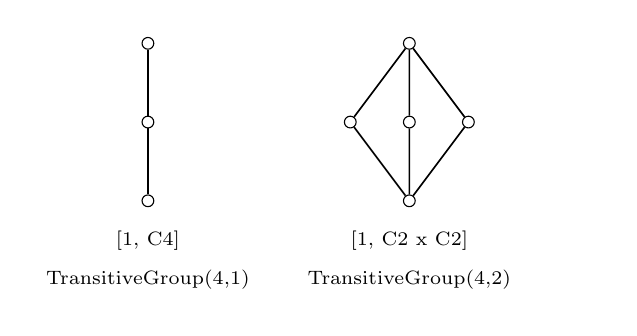
\begin{tikzpicture}[scale=.5]
\matrix[column sep=5mm,row sep=5mm]
{
\node (0) at (0,0) [draw, circle,inner sep=1.5pt] {};
\node (1) at (-0,1) [draw, circle, inner sep=1.5pt] {};
\node (2) at (-0,2) [draw, circle, inner sep=1.5pt] {};
\draw[font=\scriptsize] (0,-.5) node {[1, C4]};
\draw[font=\scriptsize] (0,-1) node {TransitiveGroup(4,1) };

\draw[semithick]
(0) to (1)
(1) to (2);
&
\node (0) at (0,0) [draw, circle,inner sep=1.5pt] {};
\node (1) at (-0,1) [draw, circle, inner sep=1.5pt] {};
\node (2) at (0.75,1) [draw, circle, inner sep=1.5pt] {};
\node (3) at (-0.75,1) [draw, circle, inner sep=1.5pt] {};
\node (4) at (-0,2) [draw, circle, inner sep=1.5pt] {};
\draw[font=\scriptsize] (0,-.5) node {[1, C2 x C2]};
\draw[font=\scriptsize] (0,-1) node {TransitiveGroup(4,2) };

\draw[semithick]
(0) to (1)
(0) to (2)
(0) to (3)
(1) to (4)
(2) to (4)
(3) to (4);
&
& \\
};
\end{tikzpicture}
\end{center}
\end{figure}



%% \input{TransitiveGsetCongEx6.tex}
\begin{figure}[h]
\caption{Transitive G-set congruence lattices in Eq(6)}
\label{fig:6}
\begin{center}
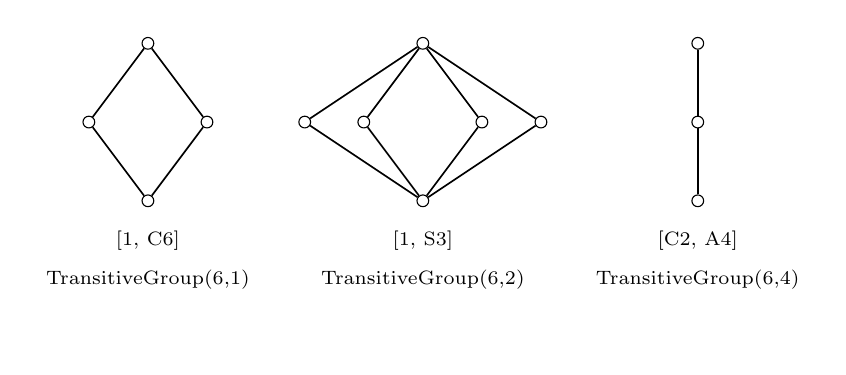
\begin{tikzpicture}[scale=.5]
\matrix[column sep=5mm,row sep=5mm]
{
\node (0) at (0,0) [draw, circle,inner sep=1.5pt] {};
\node (1) at (0.75,1) [draw, circle, inner sep=1.5pt] {};
\node (2) at (-0.75,1) [draw, circle, inner sep=1.5pt] {};
\node (3) at (-0,2) [draw, circle, inner sep=1.5pt] {};
\draw[font=\scriptsize] (0,-.5) node {[1, C6]};
\draw[font=\scriptsize] (0,-1) node {TransitiveGroup(6,1) };

\draw[semithick]
(0) to (1)
(0) to (2)
(1) to (3)
(2) to (3);
&
\node (0) at (0,0) [draw, circle,inner sep=1.5pt] {};
\node (1) at (0.75,1) [draw, circle, inner sep=1.5pt] {};
\node (2) at (-0.75,1) [draw, circle, inner sep=1.5pt] {};
\node (3) at (1.5,1) [draw, circle, inner sep=1.5pt] {};
\node (4) at (-1.5,1) [draw, circle, inner sep=1.5pt] {};
\node (5) at (-0,2) [draw, circle, inner sep=1.5pt] {};
\draw[font=\scriptsize] (0,-.5) node {[1, S3]};
\draw[font=\scriptsize] (0,-1) node {TransitiveGroup(6,2) };

\draw[semithick]
(0) to (1)
(0) to (2)
(0) to (3)
(0) to (4)
(1) to (5)
(2) to (5)
(3) to (5)
(4) to (5);
&
\node (0) at (0,0) [draw, circle,inner sep=1.5pt] {};
\node (1) at (-0,1) [draw, circle, inner sep=1.5pt] {};
\node (2) at (-0,2) [draw, circle, inner sep=1.5pt] {};
\draw[font=\scriptsize] (0,-.5) node {[C2, A4]};
\draw[font=\scriptsize] (0,-1) node {TransitiveGroup(6,4) };

\draw[semithick]
(0) to (1)
(1) to (2);
\\
\\
};
\end{tikzpicture}
\end{center}
\end{figure}

\newpage


%\input{TransitiveGsetCongEx8.tex}
\begin{figure}[h]
\caption{Transitive G-set congruence lattices in Eq(8)}
\label{fig:8}
\begin{center}
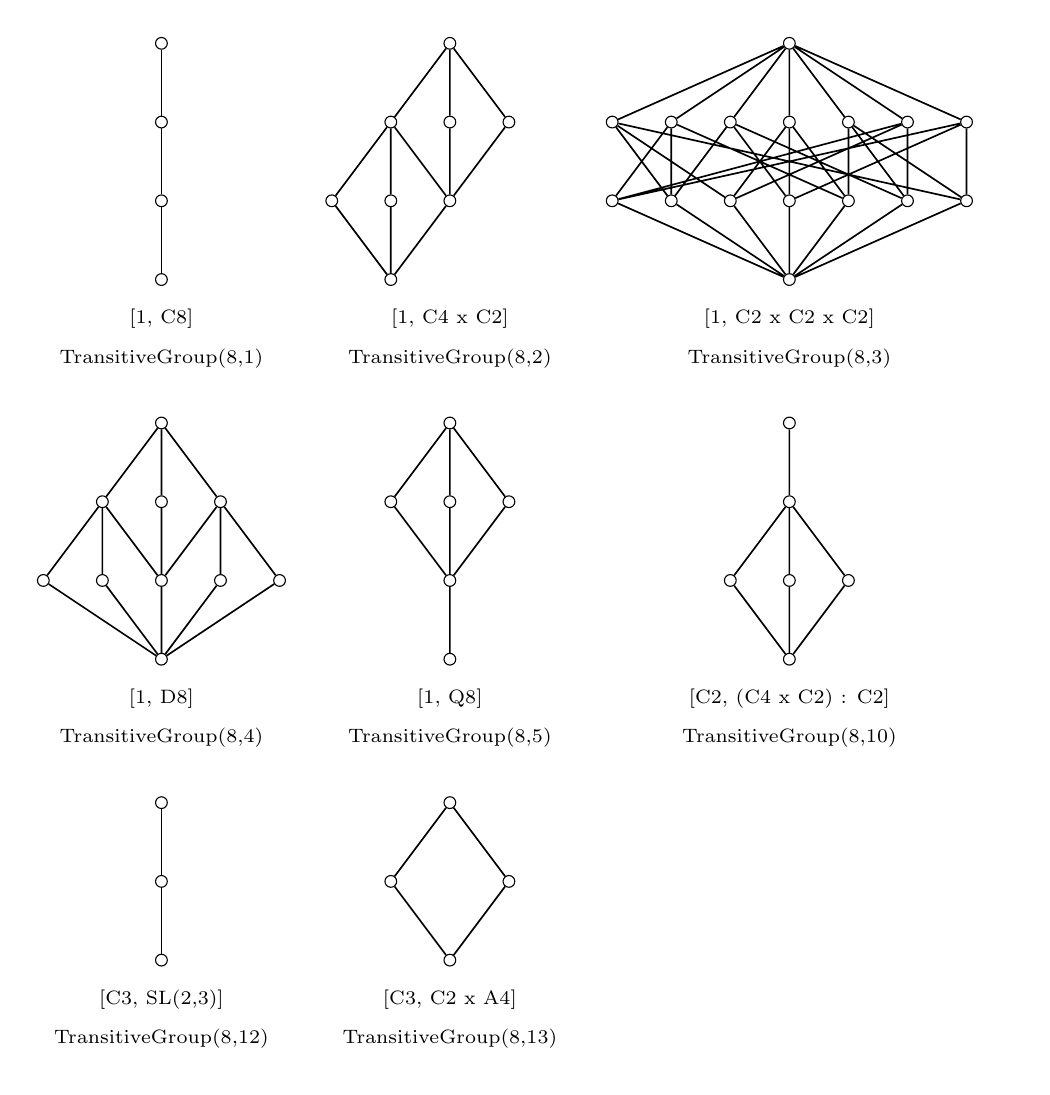
\begin{tikzpicture}[scale=.5]
\matrix[column sep=5mm,row sep=5mm]
{
\node (0) at (0,0) [draw, circle,inner sep=1.5pt] {};
\node (1) at (-0,1) [draw, circle, inner sep=1.5pt] {};
\node (2) at (-0,2) [draw, circle, inner sep=1.5pt] {};
\node (3) at (-0,3) [draw, circle, inner sep=1.5pt] {};
\draw[font=\scriptsize] (0,-.5) node {[1, C8]};
\draw[font=\scriptsize] (0,-1) node {TransitiveGroup(8,1) };

\draw[semithick]
(0) to (1)
(1) to (2)
(2) to (3);
&
%\node (0) at (0,0) [draw, circle,inner sep=1.5pt] {};
\node (0) at (-0.75,0) [draw, circle,inner sep=1.5pt] {};
\node (1) at (-0,1) [draw, circle, inner sep=1.5pt] {};
%\node (2) at (0.75,1) [draw, circle, inner sep=1.5pt] {};
\node (2) at (-1.5,1) [draw, circle, inner sep=1.5pt] {};
\node (3) at (-0.75,1) [draw, circle, inner sep=1.5pt] {};
%\node (4) at (-0,2) [draw, circle, inner sep=1.5pt] {};
\node (4) at (-0.75,2) [draw, circle, inner sep=1.5pt] {};
\node (5) at (0.75,2) [draw, circle, inner sep=1.5pt] {};
%\node (6) at (-0.75,2) [draw, circle, inner sep=1.5pt] {};
\node (6) at (0,2) [draw, circle, inner sep=1.5pt] {};
\node (7) at (-0,3) [draw, circle, inner sep=1.5pt] {};
\draw[font=\scriptsize] (0,-.5) node {[1, C4 x C2]};
\draw[font=\scriptsize] (0,-1) node {TransitiveGroup(8,2) };

\draw[semithick]
(0) to (1)
(0) to (2)
(0) to (3)
(1) to (4)
(1) to (5)
(1) to (6)
(2) to (4)
(3) to (4)
(4) to (7)
(5) to (7)
(6) to (7);
&
\node (0) at (0,0) [draw, circle,inner sep=1.5pt] {};
\node (1) at (-0,1) [draw, circle, inner sep=1.5pt] {};
\node (2) at (0.75,1) [draw, circle, inner sep=1.5pt] {};
\node (3) at (-0.75,1) [draw, circle, inner sep=1.5pt] {};
\node (4) at (1.5,1) [draw, circle, inner sep=1.5pt] {};
\node (5) at (-1.5,1) [draw, circle, inner sep=1.5pt] {};
\node (6) at (2.25,1) [draw, circle, inner sep=1.5pt] {};
\node (7) at (-2.25,1) [draw, circle, inner sep=1.5pt] {};
\node (8) at (-0,2) [draw, circle, inner sep=1.5pt] {};
\node (9) at (0.75,2) [draw, circle, inner sep=1.5pt] {};
\node (10) at (-0.75,2) [draw, circle, inner sep=1.5pt] {};
\node (11) at (1.5,2) [draw, circle, inner sep=1.5pt] {};
\node (12) at (-1.5,2) [draw, circle, inner sep=1.5pt] {};
\node (13) at (2.25,2) [draw, circle, inner sep=1.5pt] {};
\node (14) at (-2.25,2) [draw, circle, inner sep=1.5pt] {};
\node (15) at (-0,3) [draw, circle, inner sep=1.5pt] {};
\draw[font=\scriptsize] (0,-.5) node {[1, C2 x C2 x C2]};
\draw[font=\scriptsize] (0,-1) node {TransitiveGroup(8,3) };

\draw[semithick]
(0) to (1)
(0) to (2)
(0) to (3)
(0) to (4)
(0) to (5)
(0) to (6)
(0) to (7)
(1) to (8)
(1) to (10)
(1) to (13)
(2) to (8)
(2) to (9)
(2) to (12)
(3) to (8)
(3) to (11)
(3) to (14)
(4) to (9)
(4) to (10)
(4) to (11)
(5) to (10)
(5) to (12)
(5) to (14)
(6) to (9)
(6) to (13)
(6) to (14)
(7) to (11)
(7) to (12)
(7) to (13)
(8) to (15)
(9) to (15)
(10) to (15)
(11) to (15)
(12) to (15)
(13) to (15)
(14) to (15);
\\
\node (0) at (0,0) [draw, circle,inner sep=1.5pt] {};
\node (1) at (-0,1) [draw, circle, inner sep=1.5pt] {};
\node (2) at (0.75,1) [draw, circle, inner sep=1.5pt] {};
% \node (3) at (-0.75,1) [draw, circle, inner sep=1.5pt] {};
% \node (4) at (1.5,1) [draw, circle, inner sep=1.5pt] {};
\node (3) at (1.5,1) [draw, circle, inner sep=1.5pt] {};
\node (4) at (-0.75,1) [draw, circle, inner sep=1.5pt] {};
\node (5) at (-1.5,1) [draw, circle, inner sep=1.5pt] {};
% \node (6) at (-0,2) [draw, circle, inner sep=1.5pt] {};
% \node (7) at (0.75,2) [draw, circle, inner sep=1.5pt] {};
\node (6) at (0.75,2) [draw, circle, inner sep=1.5pt] {};
\node (7) at (0,2) [draw, circle, inner sep=1.5pt] {};
\node (8) at (-0.75,2) [draw, circle, inner sep=1.5pt] {};
\node (9) at (-0,3) [draw, circle, inner sep=1.5pt] {};
\draw[font=\scriptsize] (0,-.5) node {[1, D8]};
\draw[font=\scriptsize] (0,-1) node {TransitiveGroup(8,4) };

\draw[semithick]
(0) to (1)
(0) to (2)
(0) to (3)
(0) to (4)
(0) to (5)
(1) to (6)
(1) to (7)
(1) to (8)
(2) to (6)
(3) to (6)
(4) to (8)
(5) to (8)
(6) to (9)
(7) to (9)
(8) to (9);
&
\node (0) at (0,0) [draw, circle,inner sep=1.5pt] {};
\node (1) at (-0,1) [draw, circle, inner sep=1.5pt] {};
\node (2) at (-0,2) [draw, circle, inner sep=1.5pt] {};
\node (3) at (0.75,2) [draw, circle, inner sep=1.5pt] {};
\node (4) at (-0.75,2) [draw, circle, inner sep=1.5pt] {};
\node (5) at (-0,3) [draw, circle, inner sep=1.5pt] {};
\draw[font=\scriptsize] (0,-.5) node {[1, Q8]};
\draw[font=\scriptsize] (0,-1) node {TransitiveGroup(8,5) };

\draw[semithick]
(0) to (1)
(1) to (2)
(1) to (3)
(1) to (4)
(2) to (5)
(3) to (5)
(4) to (5);
&
\node (0) at (0,0) [draw, circle,inner sep=1.5pt] {};
\node (1) at (-0,1) [draw, circle, inner sep=1.5pt] {};
\node (2) at (0.75,1) [draw, circle, inner sep=1.5pt] {};
\node (3) at (-0.75,1) [draw, circle, inner sep=1.5pt] {};
\node (4) at (-0,2) [draw, circle, inner sep=1.5pt] {};
\node (5) at (-0,3) [draw, circle, inner sep=1.5pt] {};
\draw[font=\scriptsize] (0,-.5) node {[C2, (C4 x C2) : C2]};
\draw[font=\scriptsize] (0,-1) node {TransitiveGroup(8,10) };

\draw[semithick]
(0) to (1)
(0) to (2)
(0) to (3)
(1) to (4)
(2) to (4)
(3) to (4)
(4) to (5);
\\
\node (0) at (0,0) [draw, circle,inner sep=1.5pt] {};
\node (1) at (-0,1) [draw, circle, inner sep=1.5pt] {};
\node (2) at (-0,2) [draw, circle, inner sep=1.5pt] {};
\draw[font=\scriptsize] (0,-.5) node {[C3, SL(2,3)]};
\draw[font=\scriptsize] (0,-1) node {TransitiveGroup(8,12) };

\draw[semithick]
(0) to (1)
(1) to (2);
&
\node (0) at (0,0) [draw, circle,inner sep=1.5pt] {};
\node (1) at (0.75,1) [draw, circle, inner sep=1.5pt] {};
\node (2) at (-0.75,1) [draw, circle, inner sep=1.5pt] {};
\node (3) at (-0,2) [draw, circle, inner sep=1.5pt] {};
\draw[font=\scriptsize] (0,-.5) node {[C3, C2 x A4]};
\draw[font=\scriptsize] (0,-1) node {TransitiveGroup(8,13) };

\draw[semithick]
(0) to (1)
(0) to (2)
(1) to (3)
(2) to (3);
&
& \\
};
\end{tikzpicture}
\end{center}
\end{figure}

\newpage

%% \input{TransitiveGsetCongEx9.tex}
\begin{figure}[h]
\caption{Transitive G-set congruence lattices in Eq(9)}
\label{fig:9}
\begin{center}
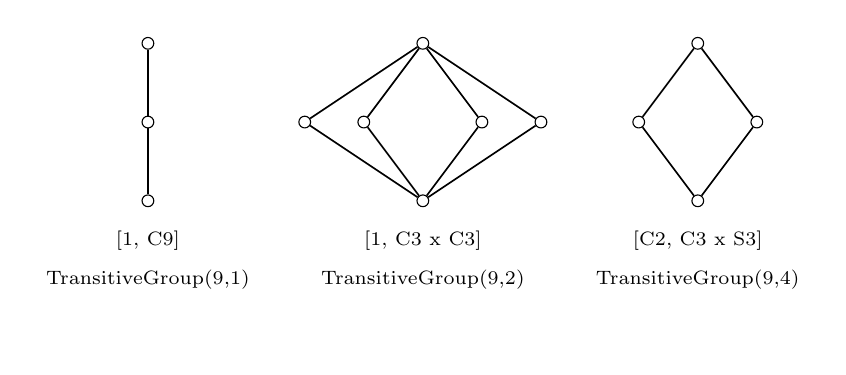
\begin{tikzpicture}[scale=.5]
\matrix[column sep=5mm,row sep=5mm]
{
\node (0) at (0,0) [draw, circle,inner sep=1.5pt] {};
\node (1) at (-0,1) [draw, circle, inner sep=1.5pt] {};
\node (2) at (-0,2) [draw, circle, inner sep=1.5pt] {};
\draw[font=\scriptsize] (0,-.5) node {[1, C9]};
\draw[font=\scriptsize] (0,-1) node {TransitiveGroup(9,1) };

\draw[semithick]
(0) to (1)
(1) to (2);
&
\node (0) at (0,0) [draw, circle,inner sep=1.5pt] {};
\node (1) at (0.75,1) [draw, circle, inner sep=1.5pt] {};
\node (2) at (-0.75,1) [draw, circle, inner sep=1.5pt] {};
\node (3) at (1.5,1) [draw, circle, inner sep=1.5pt] {};
\node (4) at (-1.5,1) [draw, circle, inner sep=1.5pt] {};
\node (5) at (-0,2) [draw, circle, inner sep=1.5pt] {};
\draw[font=\scriptsize] (0,-.5) node {[1, C3 x C3]};
\draw[font=\scriptsize] (0,-1) node {TransitiveGroup(9,2) };

\draw[semithick]
(0) to (1)
(0) to (2)
(0) to (3)
(0) to (4)
(1) to (5)
(2) to (5)
(3) to (5)
(4) to (5);
&
\node (0) at (0,0) [draw, circle,inner sep=1.5pt] {};
\node (1) at (0.75,1) [draw, circle, inner sep=1.5pt] {};
\node (2) at (-0.75,1) [draw, circle, inner sep=1.5pt] {};
\node (3) at (-0,2) [draw, circle, inner sep=1.5pt] {};
\draw[font=\scriptsize] (0,-.5) node {[C2, C3 x S3]};
\draw[font=\scriptsize] (0,-1) node {TransitiveGroup(9,4) };

\draw[semithick]
(0) to (1)
(0) to (2)
(1) to (3)
(2) to (3);
\\
\\
};
\end{tikzpicture}
\end{center}
\end{figure}

\newpage





%% \input{TransitiveGsetCongEx10.tex}
\begin{figure}[h]
\caption{Transitive G-set congruence lattices in Eq(10)}
\label{fig:10}
\begin{center}
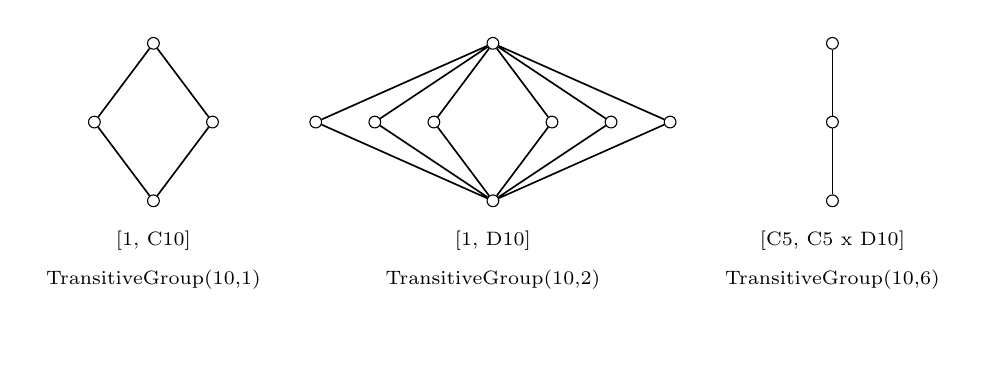
\begin{tikzpicture}[scale=.5]
\matrix[column sep=5mm,row sep=5mm]
{
\node (0) at (0,0) [draw, circle,inner sep=1.5pt] {};
\node (1) at (0.75,1) [draw, circle, inner sep=1.5pt] {};
\node (2) at (-0.75,1) [draw, circle, inner sep=1.5pt] {};
\node (3) at (-0,2) [draw, circle, inner sep=1.5pt] {};
\draw[font=\scriptsize] (0,-.5) node {[1, C10]};
\draw[font=\scriptsize] (0,-1) node {TransitiveGroup(10,1) };

\draw[semithick]
(0) to (1)
(0) to (2)
(1) to (3)
(2) to (3);
&
\node (0) at (0,0) [draw, circle,inner sep=1.5pt] {};
\node (1) at (0.75,1) [draw, circle, inner sep=1.5pt] {};
\node (2) at (-0.75,1) [draw, circle, inner sep=1.5pt] {};
\node (3) at (1.5,1) [draw, circle, inner sep=1.5pt] {};
\node (4) at (-1.5,1) [draw, circle, inner sep=1.5pt] {};
\node (5) at (2.25,1) [draw, circle, inner sep=1.5pt] {};
\node (6) at (-2.25,1) [draw, circle, inner sep=1.5pt] {};
\node (7) at (-0,2) [draw, circle, inner sep=1.5pt] {};
\draw[font=\scriptsize] (0,-.5) node {[1, D10]};
\draw[font=\scriptsize] (0,-1) node {TransitiveGroup(10,2) };

\draw[semithick]
(0) to (1)
(0) to (2)
(0) to (3)
(0) to (4)
(0) to (5)
(0) to (6)
(1) to (7)
(2) to (7)
(3) to (7)
(4) to (7)
(5) to (7)
(6) to (7);
&
\node (0) at (0,0) [draw, circle,inner sep=1.5pt] {};
\node (1) at (-0,1) [draw, circle, inner sep=1.5pt] {};
\node (2) at (-0,2) [draw, circle, inner sep=1.5pt] {};
\draw[font=\scriptsize] (0,-.5) node {[C5, C5 x D10]};
\draw[font=\scriptsize] (0,-1) node {TransitiveGroup(10,6) };

\draw[semithick]
(0) to (1)
(1) to (2);
\\
\\
};
\end{tikzpicture}
\end{center}
\end{figure}

\newpage


%% \input{TransitiveGsetCongEx12.tex}
\begin{figure}[h]
\caption{Transitive G-set congruence lattices in Eq(12)}
\label{fig:12}
\begin{center}
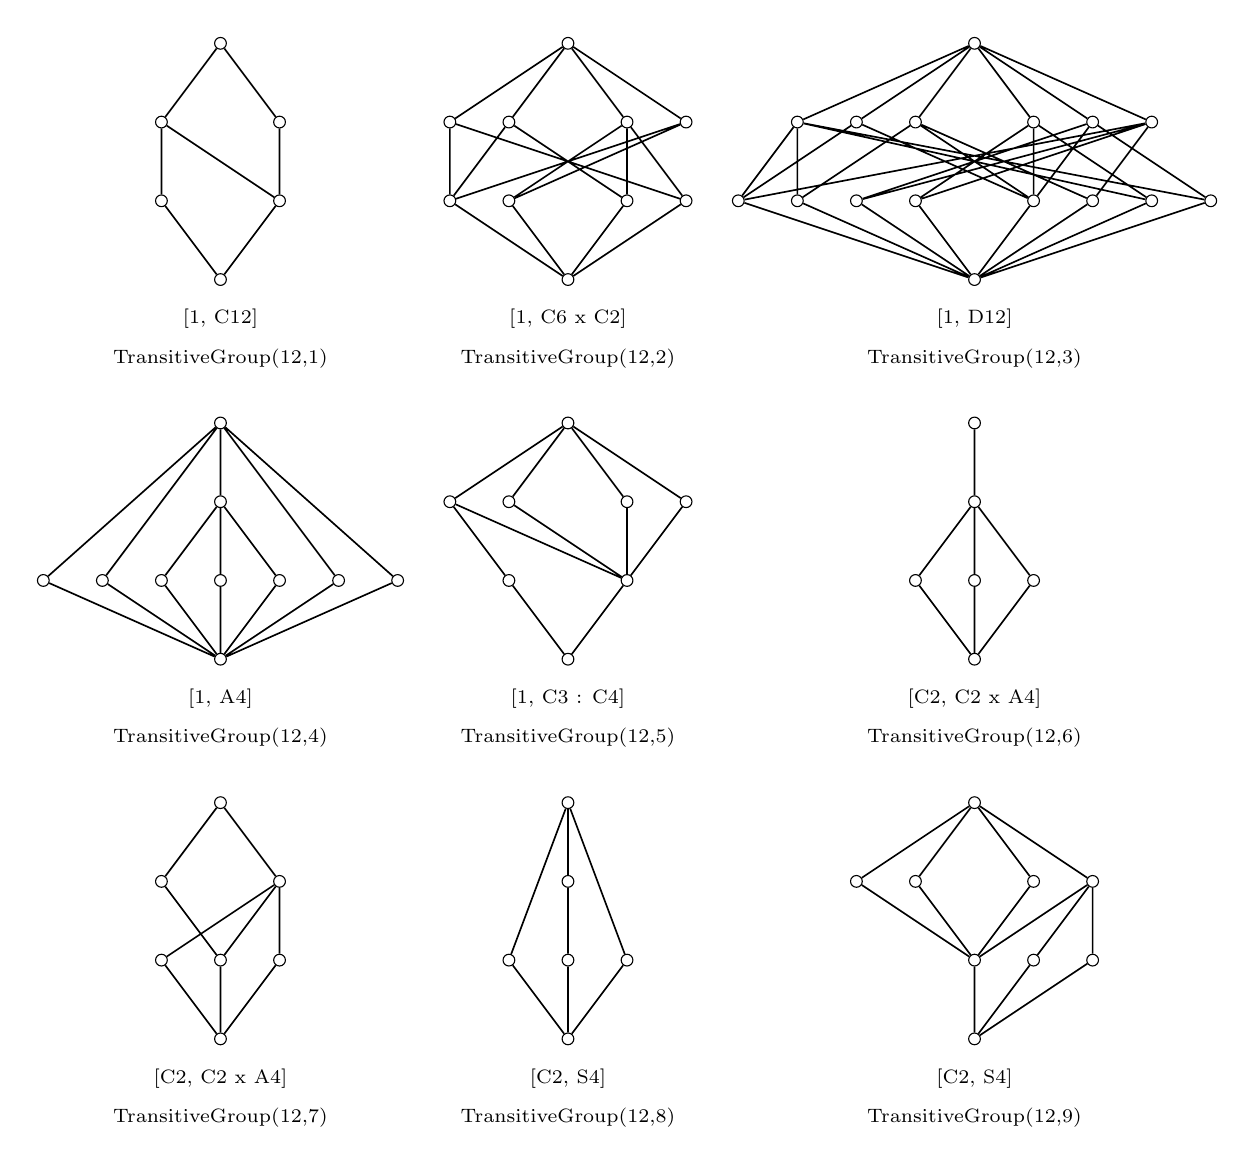
\begin{tikzpicture}[scale=.5]
\matrix[column sep=5mm,row sep=5mm]
{
\node (0) at (0,0) [draw, circle,inner sep=1.5pt] {};
\node (1) at (0.75,1) [draw, circle, inner sep=1.5pt] {};
\node (2) at (-0.75,1) [draw, circle, inner sep=1.5pt] {};
\node (3) at (0.75,2) [draw, circle, inner sep=1.5pt] {};
\node (4) at (-0.75,2) [draw, circle, inner sep=1.5pt] {};
\node (5) at (-0,3) [draw, circle, inner sep=1.5pt] {};
\draw[font=\scriptsize] (0,-.5) node {[1, C12]};
\draw[font=\scriptsize] (0,-1) node {TransitiveGroup(12,1) };

\draw[semithick]
(0) to (1)
(0) to (2)
(1) to (3)
(1) to (4)
(2) to (4)
(3) to (5)
(4) to (5);
&
\node (0) at (0,0) [draw, circle,inner sep=1.5pt] {};
\node (1) at (0.75,1) [draw, circle, inner sep=1.5pt] {};
\node (2) at (-0.75,1) [draw, circle, inner sep=1.5pt] {};
\node (3) at (1.5,1) [draw, circle, inner sep=1.5pt] {};
\node (4) at (-1.5,1) [draw, circle, inner sep=1.5pt] {};
\node (5) at (0.75,2) [draw, circle, inner sep=1.5pt] {};
\node (6) at (-0.75,2) [draw, circle, inner sep=1.5pt] {};
\node (7) at (1.5,2) [draw, circle, inner sep=1.5pt] {};
\node (8) at (-1.5,2) [draw, circle, inner sep=1.5pt] {};
\node (9) at (-0,3) [draw, circle, inner sep=1.5pt] {};
\draw[font=\scriptsize] (0,-.5) node {[1, C6 x C2]};
\draw[font=\scriptsize] (0,-1) node {TransitiveGroup(12,2) };

\draw[semithick]
(0) to (1)
(0) to (2)
(0) to (3)
(0) to (4)
(1) to (5)
(1) to (6)
(2) to (5)
(2) to (7)
(3) to (5)
(3) to (8)
(4) to (6)
(4) to (7)
(4) to (8)
(5) to (9)
(6) to (9)
(7) to (9)
(8) to (9);
&
\node (0) at (0,0) [draw, circle,inner sep=1.5pt] {};
\node (1) at (0.75,1) [draw, circle, inner sep=1.5pt] {};
\node (2) at (-0.75,1) [draw, circle, inner sep=1.5pt] {};
\node (3) at (1.5,1) [draw, circle, inner sep=1.5pt] {};
\node (4) at (-1.5,1) [draw, circle, inner sep=1.5pt] {};
\node (5) at (2.25,1) [draw, circle, inner sep=1.5pt] {};
\node (6) at (-2.25,1) [draw, circle, inner sep=1.5pt] {};
\node (7) at (3,1) [draw, circle, inner sep=1.5pt] {};
\node (8) at (-3,1) [draw, circle, inner sep=1.5pt] {};
\node (9) at (0.75,2) [draw, circle, inner sep=1.5pt] {};
\node (10) at (-0.75,2) [draw, circle, inner sep=1.5pt] {};
\node (11) at (1.5,2) [draw, circle, inner sep=1.5pt] {};
\node (12) at (-1.5,2) [draw, circle, inner sep=1.5pt] {};
\node (13) at (2.25,2) [draw, circle, inner sep=1.5pt] {};
\node (14) at (-2.25,2) [draw, circle, inner sep=1.5pt] {};
\node (15) at (-0,3) [draw, circle, inner sep=1.5pt] {};
\draw[font=\scriptsize] (0,-.5) node {[1, D12]};
\draw[font=\scriptsize] (0,-1) node {TransitiveGroup(12,3) };

\draw[semithick]
(0) to (1)
(0) to (2)
(0) to (3)
(0) to (4)
(0) to (5)
(0) to (6)
(0) to (7)
(0) to (8)
(1) to (9)
(1) to (10)
(1) to (11)
(1) to (12)
(2) to (9)
(2) to (13)
(3) to (10)
(3) to (13)
(4) to (11)
(4) to (13)
(5) to (9)
(5) to (14)
(6) to (10)
(6) to (14)
(7) to (11)
(7) to (14)
(8) to (12)
(8) to (13)
(8) to (14)
(9) to (15)
(10) to (15)
(11) to (15)
(12) to (15)
(13) to (15)
(14) to (15);
\\
\node (0) at (0,0) [draw, circle,inner sep=1.5pt] {};
\node (1) at (-0,1) [draw, circle, inner sep=1.5pt] {};
\node (2) at (0.75,1) [draw, circle, inner sep=1.5pt] {};
\node (3) at (-0.75,1) [draw, circle, inner sep=1.5pt] {};
\node (4) at (1.5,1) [draw, circle, inner sep=1.5pt] {};
\node (5) at (-1.5,1) [draw, circle, inner sep=1.5pt] {};
\node (6) at (2.25,1) [draw, circle, inner sep=1.5pt] {};
\node (7) at (-2.25,1) [draw, circle, inner sep=1.5pt] {};
\node (8) at (-0,2) [draw, circle, inner sep=1.5pt] {};
\node (9) at (-0,3) [draw, circle, inner sep=1.5pt] {};
\draw[font=\scriptsize] (0,-.5) node {[1, A4]};
\draw[font=\scriptsize] (0,-1) node {TransitiveGroup(12,4) };

\draw[semithick]
(0) to (1)
(0) to (2)
(0) to (3)
(0) to (4)
(0) to (5)
(0) to (6)
(0) to (7)
(1) to (8)
(2) to (8)
(3) to (8)
(4) to (9)
(5) to (9)
(6) to (9)
(7) to (9)
(8) to (9);
&
\node (0) at (0,0) [draw, circle,inner sep=1.5pt] {};
\node (1) at (0.75,1) [draw, circle, inner sep=1.5pt] {};
\node (2) at (-0.75,1) [draw, circle, inner sep=1.5pt] {};
\node (3) at (0.75,2) [draw, circle, inner sep=1.5pt] {};
\node (4) at (-0.75,2) [draw, circle, inner sep=1.5pt] {};
\node (5) at (1.5,2) [draw, circle, inner sep=1.5pt] {};
\node (6) at (-1.5,2) [draw, circle, inner sep=1.5pt] {};
\node (7) at (-0,3) [draw, circle, inner sep=1.5pt] {};
\draw[font=\scriptsize] (0,-.5) node {[1, C3 : C4]};
\draw[font=\scriptsize] (0,-1) node {TransitiveGroup(12,5) };

\draw[semithick]
(0) to (1)
(0) to (2)
(1) to (3)
(1) to (4)
(1) to (5)
(1) to (6)
(2) to (6)
(3) to (7)
(4) to (7)
(5) to (7)
(6) to (7);
&
\node (0) at (0,0) [draw, circle,inner sep=1.5pt] {};
\node (1) at (-0,1) [draw, circle, inner sep=1.5pt] {};
\node (2) at (0.75,1) [draw, circle, inner sep=1.5pt] {};
\node (3) at (-0.75,1) [draw, circle, inner sep=1.5pt] {};
\node (4) at (-0,2) [draw, circle, inner sep=1.5pt] {};
\node (5) at (-0,3) [draw, circle, inner sep=1.5pt] {};
\draw[font=\scriptsize] (0,-.5) node {[C2, C2 x A4]};
\draw[font=\scriptsize] (0,-1) node {TransitiveGroup(12,6) };

\draw[semithick]
(0) to (1)
(0) to (2)
(0) to (3)
(1) to (4)
(2) to (4)
(3) to (4)
(4) to (5);
\\
\node (0) at (0,0) [draw, circle,inner sep=1.5pt] {};
\node (1) at (-0,1) [draw, circle, inner sep=1.5pt] {};
\node (2) at (0.75,1) [draw, circle, inner sep=1.5pt] {};
\node (3) at (-0.75,1) [draw, circle, inner sep=1.5pt] {};
\node (4) at (0.75,2) [draw, circle, inner sep=1.5pt] {};
\node (5) at (-0.75,2) [draw, circle, inner sep=1.5pt] {};
\node (6) at (-0,3) [draw, circle, inner sep=1.5pt] {};
\draw[font=\scriptsize] (0,-.5) node {[C2, C2 x A4]};
\draw[font=\scriptsize] (0,-1) node {TransitiveGroup(12,7) };

\draw[semithick]
(0) to (1)
(0) to (2)
(0) to (3)
(1) to (4)
(1) to (5)
(2) to (4)
(3) to (4)
(4) to (6)
(5) to (6);
&
\node (0) at (0,0) [draw, circle,inner sep=1.5pt] {};
\node (1) at (-0,1) [draw, circle, inner sep=1.5pt] {};
\node (2) at (0.75,1) [draw, circle, inner sep=1.5pt] {};
\node (3) at (-0.75,1) [draw, circle, inner sep=1.5pt] {};
\node (4) at (-0,2) [draw, circle, inner sep=1.5pt] {};
\node (5) at (-0,3) [draw, circle, inner sep=1.5pt] {};
\draw[font=\scriptsize] (0,-.5) node {[C2, S4]};
\draw[font=\scriptsize] (0,-1) node {TransitiveGroup(12,8) };

\draw[semithick]
(0) to (1)
(0) to (2)
(0) to (3)
(1) to (4)
(2) to (5)
(3) to (5)
(4) to (5);
&
 \node (0) at (0,0) [draw, circle,inner sep=1.5pt] {};
% \node (1) at (-0,1) [draw, circle, inner sep=1.5pt] {};
% \node (2) at (0.75,1) [draw, circle, inner sep=1.5pt] {};
% \node (3) at (-0.75,1) [draw, circle, inner sep=1.5pt] {};
%\node (0) at (0.75,0) [draw, circle,inner sep=1.5pt] {};
\node (1) at (0.75,1) [draw, circle, inner sep=1.5pt] {};
\node (2) at (1.5,1) [draw, circle, inner sep=1.5pt] {};
\node (3) at (0,1) [draw, circle, inner sep=1.5pt] {};
\node (4) at (0.75,2) [draw, circle, inner sep=1.5pt] {};
\node (5) at (-0.75,2) [draw, circle, inner sep=1.5pt] {};
\node (6) at (1.5,2) [draw, circle, inner sep=1.5pt] {};
\node (7) at (-1.5,2) [draw, circle, inner sep=1.5pt] {};
\node (8) at (-0,3) [draw, circle, inner sep=1.5pt] {};
\draw[font=\scriptsize] (0,-.5) node {[C2, S4]};
\draw[font=\scriptsize] (0,-1) node {TransitiveGroup(12,9) };

\draw[semithick]
(0) to (1)
(0) to (2)
(0) to (3)
(1) to (6)
(2) to (6)
(3) to (4)
(3) to (5)
(3) to (6)
(3) to (7)
(4) to (8)
(5) to (8)
(6) to (8)
(7) to (8);
\\
};
\end{tikzpicture}
\end{center}
\end{figure}

\newpage

\begin{figure}[h]
\caption{Transitive G-set congruence lattices in Eq(12) (continued)}
\label{fig:12b}
\begin{center}
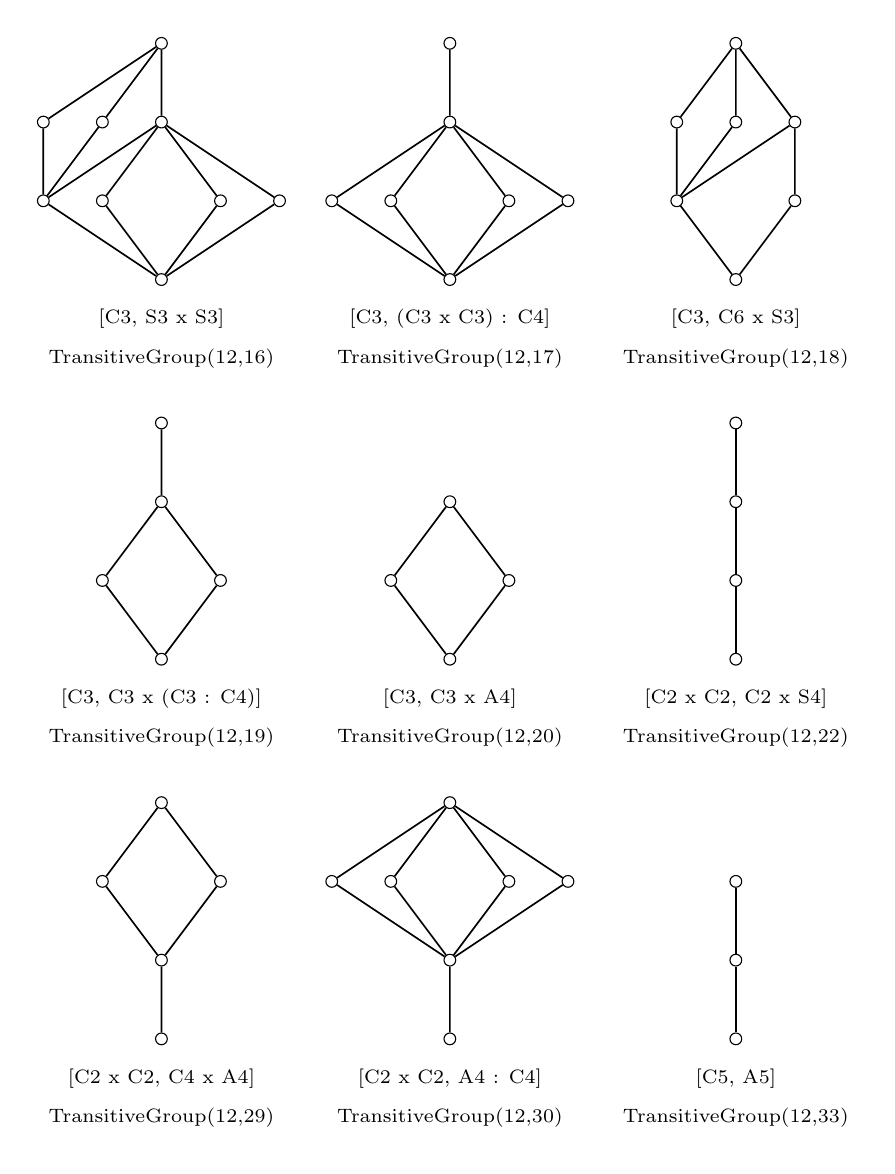
\begin{tikzpicture}[scale=.5]
\matrix[column sep=5mm,row sep=5mm]
{
\node (0) at (0,0) [draw, circle,inner sep=1.5pt] {};
\node (1) at (0.75,1) [draw, circle, inner sep=1.5pt] {};
\node (2) at (-0.75,1) [draw, circle, inner sep=1.5pt] {};
\node (3) at (1.5,1) [draw, circle, inner sep=1.5pt] {};
\node (4) at (-1.5,1) [draw, circle, inner sep=1.5pt] {};
% \node (5) at (-0,2) [draw, circle, inner sep=1.5pt] {};
% \node (6) at (0.75,2) [draw, circle, inner sep=1.5pt] {};
% \node (7) at (-0.75,2) [draw, circle, inner sep=1.5pt] {};
\node (5) at (-0.75,2) [draw, circle, inner sep=1.5pt] {};
\node (6) at (-1.5,2) [draw, circle, inner sep=1.5pt] {};
\node (7) at (0,2) [draw, circle, inner sep=1.5pt] {};
\node (8) at (-0,3) [draw, circle, inner sep=1.5pt] {};
\draw[font=\scriptsize] (0,-.5) node {[C3, S3 x S3]};
\draw[font=\scriptsize] (0,-1) node {TransitiveGroup(12,16) };

\draw[semithick]
(0) to (1)
(0) to (2)
(0) to (3)
(0) to (4)
(1) to (7)
(2) to (7)
(3) to (7)
(4) to (5)
(4) to (6)
(4) to (7)
(5) to (8)
(6) to (8)
(7) to (8);
&
\node (0) at (0,0) [draw, circle,inner sep=1.5pt] {};
\node (1) at (0.75,1) [draw, circle, inner sep=1.5pt] {};
\node (2) at (-0.75,1) [draw, circle, inner sep=1.5pt] {};
\node (3) at (1.5,1) [draw, circle, inner sep=1.5pt] {};
\node (4) at (-1.5,1) [draw, circle, inner sep=1.5pt] {};
\node (5) at (-0,2) [draw, circle, inner sep=1.5pt] {};
\node (6) at (-0,3) [draw, circle, inner sep=1.5pt] {};
\draw[font=\scriptsize] (0,-.5) node {[C3, (C3 x C3) : C4]};
\draw[font=\scriptsize] (0,-1) node {TransitiveGroup(12,17) };

\draw[semithick]
(0) to (1)
(0) to (2)
(0) to (3)
(0) to (4)
(1) to (5)
(2) to (5)
(3) to (5)
(4) to (5)
(5) to (6);
&
\node (0) at (0,0) [draw, circle,inner sep=1.5pt] {};
\node (1) at (0.75,1) [draw, circle, inner sep=1.5pt] {};
\node (2) at (-0.75,1) [draw, circle, inner sep=1.5pt] {};
\node (3) at (-0,2) [draw, circle, inner sep=1.5pt] {};
\node (4) at (0.75,2) [draw, circle, inner sep=1.5pt] {};
\node (5) at (-0.75,2) [draw, circle, inner sep=1.5pt] {};
\node (6) at (-0,3) [draw, circle, inner sep=1.5pt] {};
\draw[font=\scriptsize] (0,-.5) node {[C3, C6 x S3]};
\draw[font=\scriptsize] (0,-1) node {TransitiveGroup(12,18) };

\draw[semithick]
(0) to (1)
(0) to (2)
(1) to (4)
(2) to (3)
(2) to (4)
(2) to (5)
(3) to (6)
(4) to (6)
(5) to (6);
\\
\node (0) at (0,0) [draw, circle,inner sep=1.5pt] {};
\node (1) at (0.75,1) [draw, circle, inner sep=1.5pt] {};
\node (2) at (-0.75,1) [draw, circle, inner sep=1.5pt] {};
\node (3) at (-0,2) [draw, circle, inner sep=1.5pt] {};
\node (4) at (-0,3) [draw, circle, inner sep=1.5pt] {};
\draw[font=\scriptsize] (0,-.5) node {[C3, C3 x (C3 : C4)]};
\draw[font=\scriptsize] (0,-1) node {TransitiveGroup(12,19) };

\draw[semithick]
(0) to (1)
(0) to (2)
(1) to (3)
(2) to (3)
(3) to (4);
&
\node (0) at (0,0) [draw, circle,inner sep=1.5pt] {};
\node (1) at (0.75,1) [draw, circle, inner sep=1.5pt] {};
\node (2) at (-0.75,1) [draw, circle, inner sep=1.5pt] {};
\node (3) at (-0,2) [draw, circle, inner sep=1.5pt] {};
\draw[font=\scriptsize] (0,-.5) node {[C3, C3 x A4]};
\draw[font=\scriptsize] (0,-1) node {TransitiveGroup(12,20) };

\draw[semithick]
(0) to (1)
(0) to (2)
(1) to (3)
(2) to (3);
&
\node (0) at (0,0) [draw, circle,inner sep=1.5pt] {};
\node (1) at (-0,1) [draw, circle, inner sep=1.5pt] {};
\node (2) at (-0,2) [draw, circle, inner sep=1.5pt] {};
\node (3) at (-0,3) [draw, circle, inner sep=1.5pt] {};
\draw[font=\scriptsize] (0,-.5) node {[C2 x C2, C2 x S4]};
\draw[font=\scriptsize] (0,-1) node {TransitiveGroup(12,22) };

\draw[semithick]
(0) to (1)
(1) to (2)
(2) to (3);
\\
\node (0) at (0,0) [draw, circle,inner sep=1.5pt] {};
\node (1) at (-0,1) [draw, circle, inner sep=1.5pt] {};
\node (2) at (0.75,2) [draw, circle, inner sep=1.5pt] {};
\node (3) at (-0.75,2) [draw, circle, inner sep=1.5pt] {};
\node (4) at (-0,3) [draw, circle, inner sep=1.5pt] {};
\draw[font=\scriptsize] (0,-.5) node {[C2 x C2, C4 x A4]};
\draw[font=\scriptsize] (0,-1) node {TransitiveGroup(12,29) };

\draw[semithick]
(0) to (1)
(1) to (2)
(1) to (3)
(2) to (4)
(3) to (4);
&
\node (0) at (0,0) [draw, circle,inner sep=1.5pt] {};
\node (1) at (-0,1) [draw, circle, inner sep=1.5pt] {};
\node (2) at (0.75,2) [draw, circle, inner sep=1.5pt] {};
\node (3) at (-0.75,2) [draw, circle, inner sep=1.5pt] {};
\node (4) at (1.5,2) [draw, circle, inner sep=1.5pt] {};
\node (5) at (-1.5,2) [draw, circle, inner sep=1.5pt] {};
\node (6) at (-0,3) [draw, circle, inner sep=1.5pt] {};
\draw[font=\scriptsize] (0,-.5) node {[C2 x C2, A4 : C4]};
\draw[font=\scriptsize] (0,-1) node {TransitiveGroup(12,30) };

\draw[semithick]
(0) to (1)
(1) to (2)
(1) to (3)
(1) to (4)
(1) to (5)
(2) to (6)
(3) to (6)
(4) to (6)
(5) to (6);
&
\node (0) at (0,0) [draw, circle,inner sep=1.5pt] {};
\node (1) at (-0,1) [draw, circle, inner sep=1.5pt] {};
\node (2) at (-0,2) [draw, circle, inner sep=1.5pt] {};
\draw[font=\scriptsize] (0,-.5) node {[C5, A5]};
\draw[font=\scriptsize] (0,-1) node {TransitiveGroup(12,33) };

\draw[semithick]
(0) to (1)
(1) to (2);
\\
};
\end{tikzpicture}
\end{center}
\end{figure}

\newpage

\begin{figure}[h]
\caption{Transitive G-set congruence lattices in Eq(12) (continued)}
\label{fig:12c}
\begin{center}
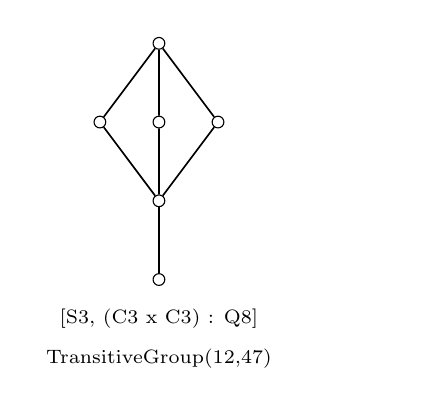
\begin{tikzpicture}[scale=.5]
\matrix[column sep=5mm,row sep=5mm]
{
\node (0) at (0,0) [draw, circle,inner sep=1.5pt] {};
\node (1) at (-0,1) [draw, circle, inner sep=1.5pt] {};
\node (2) at (-0,2) [draw, circle, inner sep=1.5pt] {};
\node (3) at (0.75,2) [draw, circle, inner sep=1.5pt] {};
\node (4) at (-0.75,2) [draw, circle, inner sep=1.5pt] {};
\node (5) at (-0,3) [draw, circle, inner sep=1.5pt] {};
\draw[font=\scriptsize] (0,-.5) node {[S3, (C3 x C3) : Q8]};
\draw[font=\scriptsize] (0,-1) node {TransitiveGroup(12,47) };

\draw[semithick]
(0) to (1)
(1) to (2)
(1) to (3)
(1) to (4)
(2) to (5)
(3) to (5)
(4) to (5);
&
& & \\
};
\end{tikzpicture}
\end{center}
\end{figure}

\newpage


%% \input{TransitiveGsetCongEx14.tex}
\begin{figure}[h]
\caption{Transitive G-set congruence lattices in Eq(14)}
\label{fig:14}
\begin{center}
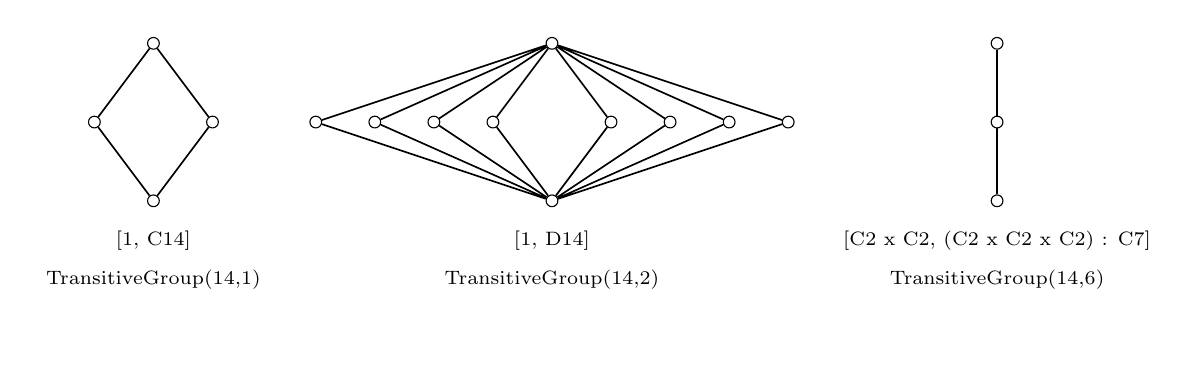
\begin{tikzpicture}[scale=.5]
\matrix[column sep=5mm,row sep=5mm]
{
\node (0) at (0,0) [draw, circle,inner sep=1.5pt] {};
\node (1) at (0.75,1) [draw, circle, inner sep=1.5pt] {};
\node (2) at (-0.75,1) [draw, circle, inner sep=1.5pt] {};
\node (3) at (-0,2) [draw, circle, inner sep=1.5pt] {};
\draw[font=\scriptsize] (0,-.5) node {[1, C14]};
\draw[font=\scriptsize] (0,-1) node {TransitiveGroup(14,1) };

\draw[semithick]
(0) to (1)
(0) to (2)
(1) to (3)
(2) to (3);
&
\node (0) at (0,0) [draw, circle,inner sep=1.5pt] {};
\node (1) at (0.75,1) [draw, circle, inner sep=1.5pt] {};
\node (2) at (-0.75,1) [draw, circle, inner sep=1.5pt] {};
\node (3) at (1.5,1) [draw, circle, inner sep=1.5pt] {};
\node (4) at (-1.5,1) [draw, circle, inner sep=1.5pt] {};
\node (5) at (2.25,1) [draw, circle, inner sep=1.5pt] {};
\node (6) at (-2.25,1) [draw, circle, inner sep=1.5pt] {};
\node (7) at (3,1) [draw, circle, inner sep=1.5pt] {};
\node (8) at (-3,1) [draw, circle, inner sep=1.5pt] {};
\node (9) at (-0,2) [draw, circle, inner sep=1.5pt] {};
\draw[font=\scriptsize] (0,-.5) node {[1, D14]};
\draw[font=\scriptsize] (0,-1) node {TransitiveGroup(14,2) };

\draw[semithick]
(0) to (1)
(0) to (2)
(0) to (3)
(0) to (4)
(0) to (5)
(0) to (6)
(0) to (7)
(0) to (8)
(1) to (9)
(2) to (9)
(3) to (9)
(4) to (9)
(5) to (9)
(6) to (9)
(7) to (9)
(8) to (9);
&
\node (0) at (0,0) [draw, circle,inner sep=1.5pt] {};
\node (1) at (-0,1) [draw, circle, inner sep=1.5pt] {};
\node (2) at (-0,2) [draw, circle, inner sep=1.5pt] {};
\draw[font=\scriptsize] (0,-.5) node {[C2 x C2, (C2 x C2 x C2) : C7]};
\draw[font=\scriptsize] (0,-1) node {TransitiveGroup(14,6) };

\draw[semithick]
(0) to (1)
(1) to (2);
\\
\\
};
\end{tikzpicture}
\end{center}
\end{figure}

\newpage


%% \input{TransitiveGsetCongEx15.tex}
\begin{figure}[h]
\caption{Transitive G-set congruence lattices in Eq(15)}
\label{fig:15}
\begin{center}
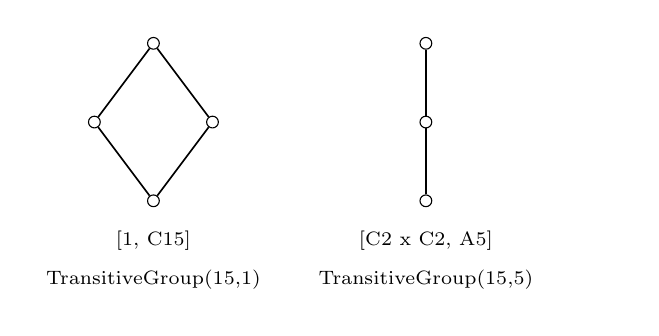
\begin{tikzpicture}[scale=.5]
\matrix[column sep=5mm,row sep=5mm]
{
\node (0) at (0,0) [draw, circle,inner sep=1.5pt] {};
\node (1) at (0.75,1) [draw, circle, inner sep=1.5pt] {};
\node (2) at (-0.75,1) [draw, circle, inner sep=1.5pt] {};
\node (3) at (-0,2) [draw, circle, inner sep=1.5pt] {};
\draw[font=\scriptsize] (0,-.5) node {[1, C15]};
\draw[font=\scriptsize] (0,-1) node {TransitiveGroup(15,1) };

\draw[semithick]
(0) to (1)
(0) to (2)
(1) to (3)
(2) to (3);
&
\node (0) at (0,0) [draw, circle,inner sep=1.5pt] {};
\node (1) at (-0,1) [draw, circle, inner sep=1.5pt] {};
\node (2) at (-0,2) [draw, circle, inner sep=1.5pt] {};
\draw[font=\scriptsize] (0,-.5) node {[C2 x C2, A5]};
\draw[font=\scriptsize] (0,-1) node {TransitiveGroup(15,5) };

\draw[semithick]
(0) to (1)
(1) to (2);
&
& \\
};
\end{tikzpicture}
\end{center}
\end{figure}

\newpage


%\input{TransitiveGsetCongEx16.tex}
%% \input{TransitiveGsetCongEx16CorefreeMin3Max10.tex}
\begin{figure}[h]
\caption{Transitive G-set congruence lattices in Eq(16)}
\label{fig:16}
\begin{center}
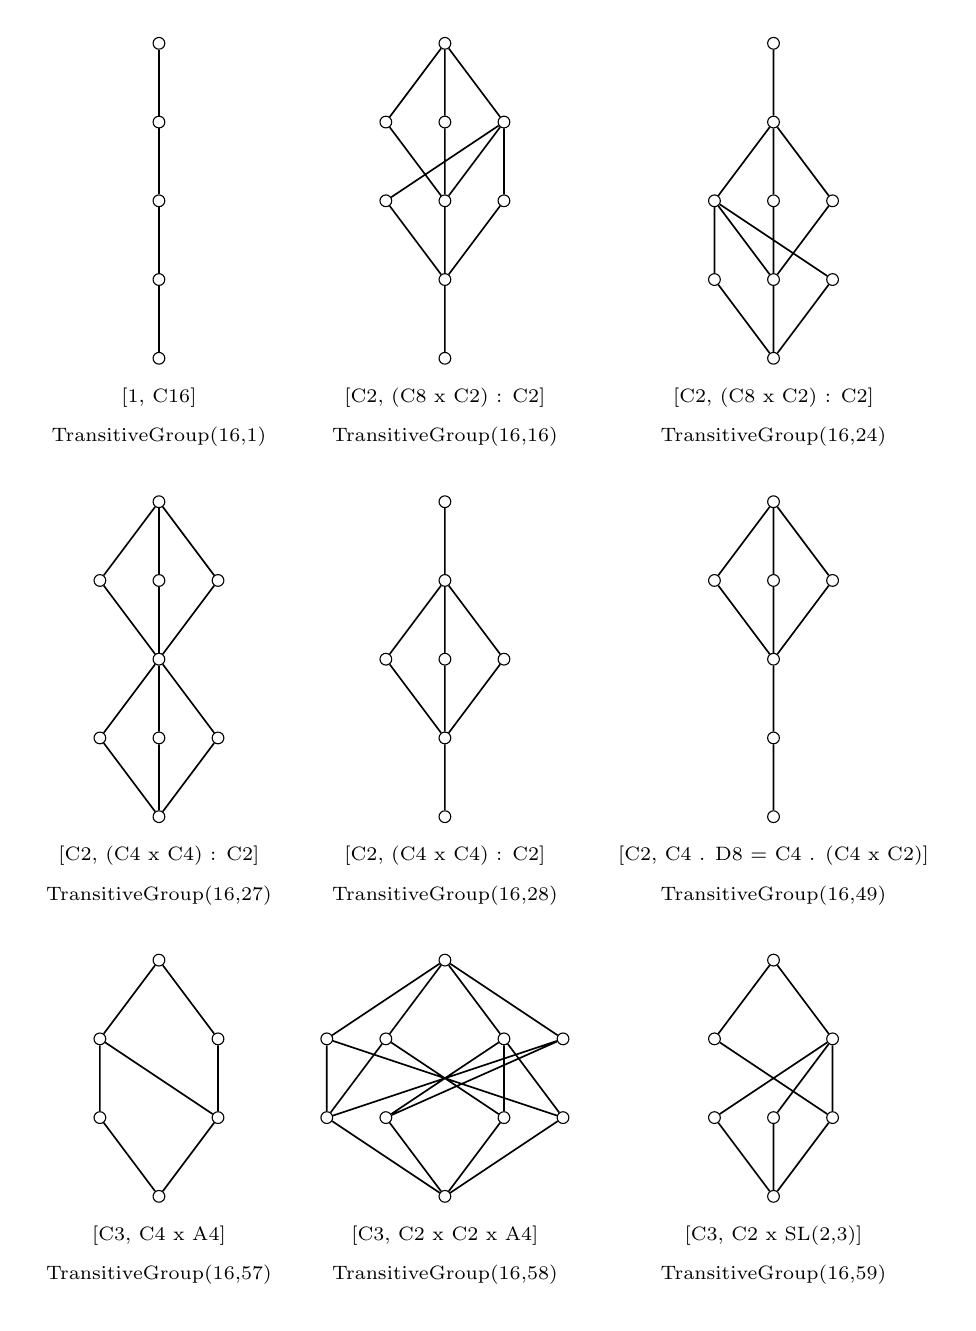
\begin{tikzpicture}[scale=.5]
\matrix[column sep=5mm,row sep=5mm]
{
\node (0) at (0,0) [draw, circle,inner sep=1.5pt] {};
\node (1) at (-0,1) [draw, circle, inner sep=1.5pt] {};
\node (2) at (-0,2) [draw, circle, inner sep=1.5pt] {};
\node (3) at (-0,3) [draw, circle, inner sep=1.5pt] {};
\node (4) at (-0,4) [draw, circle, inner sep=1.5pt] {};
\draw[font=\scriptsize] (0,-.5) node {[1, C16]};
\draw[font=\scriptsize] (0,-1) node {TransitiveGroup(16,1) };

\draw[semithick]
(0) to (1)
(1) to (2)
(2) to (3)
(3) to (4);
&
\node (0) at (0,0) [draw, circle,inner sep=1.5pt] {};
\node (1) at (-0,1) [draw, circle, inner sep=1.5pt] {};
\node (2) at (-0,2) [draw, circle, inner sep=1.5pt] {};
\node (3) at (0.75,2) [draw, circle, inner sep=1.5pt] {};
\node (4) at (-0.75,2) [draw, circle, inner sep=1.5pt] {};
\node (5) at (-0,3) [draw, circle, inner sep=1.5pt] {};
\node (6) at (0.75,3) [draw, circle, inner sep=1.5pt] {};
\node (7) at (-0.75,3) [draw, circle, inner sep=1.5pt] {};
\node (8) at (-0,4) [draw, circle, inner sep=1.5pt] {};
\draw[font=\scriptsize] (0,-.5) node {[C2, (C8 x C2) : C2]};
\draw[font=\scriptsize] (0,-1) node {TransitiveGroup(16,16) };

\draw[semithick]
(0) to (1)
(1) to (2)
(1) to (3)
(1) to (4)
(2) to (5)
(2) to (6)
(2) to (7)
(3) to (6)
(4) to (6)
(5) to (8)
(6) to (8)
(7) to (8);
&
\node (0) at (0,0) [draw, circle,inner sep=1.5pt] {};
\node (1) at (-0,1) [draw, circle, inner sep=1.5pt] {};
\node (2) at (0.75,1) [draw, circle, inner sep=1.5pt] {};
\node (3) at (-0.75,1) [draw, circle, inner sep=1.5pt] {};
\node (4) at (-0,2) [draw, circle, inner sep=1.5pt] {};
\node (5) at (0.75,2) [draw, circle, inner sep=1.5pt] {};
\node (6) at (-0.75,2) [draw, circle, inner sep=1.5pt] {};
\node (7) at (-0,3) [draw, circle, inner sep=1.5pt] {};
\node (8) at (-0,4) [draw, circle, inner sep=1.5pt] {};
\draw[font=\scriptsize] (0,-.5) node {[C2, (C8 x C2) : C2]};
\draw[font=\scriptsize] (0,-1) node {TransitiveGroup(16,24) };

\draw[semithick]
(0) to (1)
(0) to (2)
(0) to (3)
(1) to (4)
(1) to (5)
(1) to (6)
(2) to (6)
(3) to (6)
(4) to (7)
(5) to (7)
(6) to (7)
(7) to (8);
\\
\node (0) at (0,0) [draw, circle,inner sep=1.5pt] {};
\node (1) at (-0,1) [draw, circle, inner sep=1.5pt] {};
\node (2) at (0.75,1) [draw, circle, inner sep=1.5pt] {};
\node (3) at (-0.75,1) [draw, circle, inner sep=1.5pt] {};
\node (4) at (-0,2) [draw, circle, inner sep=1.5pt] {};
\node (5) at (-0,3) [draw, circle, inner sep=1.5pt] {};
\node (6) at (0.75,3) [draw, circle, inner sep=1.5pt] {};
\node (7) at (-0.75,3) [draw, circle, inner sep=1.5pt] {};
\node (8) at (-0,4) [draw, circle, inner sep=1.5pt] {};
\draw[font=\scriptsize] (0,-.5) node {[C2, (C4 x C4) : C2]};
\draw[font=\scriptsize] (0,-1) node {TransitiveGroup(16,27) };

\draw[semithick]
(0) to (1)
(0) to (2)
(0) to (3)
(1) to (4)
(2) to (4)
(3) to (4)
(4) to (5)
(4) to (6)
(4) to (7)
(5) to (8)
(6) to (8)
(7) to (8);
&
\node (0) at (0,0) [draw, circle,inner sep=1.5pt] {};
\node (1) at (-0,1) [draw, circle, inner sep=1.5pt] {};
\node (2) at (-0,2) [draw, circle, inner sep=1.5pt] {};
\node (3) at (0.75,2) [draw, circle, inner sep=1.5pt] {};
\node (4) at (-0.75,2) [draw, circle, inner sep=1.5pt] {};
\node (5) at (-0,3) [draw, circle, inner sep=1.5pt] {};
\node (6) at (-0,4) [draw, circle, inner sep=1.5pt] {};
\draw[font=\scriptsize] (0,-.5) node {[C2, (C4 x C4) : C2]};
\draw[font=\scriptsize] (0,-1) node {TransitiveGroup(16,28) };

\draw[semithick]
(0) to (1)
(1) to (2)
(1) to (3)
(1) to (4)
(2) to (5)
(3) to (5)
(4) to (5)
(5) to (6);
&
\node (0) at (0,0) [draw, circle,inner sep=1.5pt] {};
\node (1) at (-0,1) [draw, circle, inner sep=1.5pt] {};
\node (2) at (-0,2) [draw, circle, inner sep=1.5pt] {};
\node (3) at (-0,3) [draw, circle, inner sep=1.5pt] {};
\node (4) at (0.75,3) [draw, circle, inner sep=1.5pt] {};
\node (5) at (-0.75,3) [draw, circle, inner sep=1.5pt] {};
\node (6) at (-0,4) [draw, circle, inner sep=1.5pt] {};
\draw[font=\scriptsize] (0,-.5) node {[C2, C4 . D8 = C4 . (C4 x C2)]};
\draw[font=\scriptsize] (0,-1) node {TransitiveGroup(16,49) };

\draw[semithick]
(0) to (1)
(1) to (2)
(2) to (3)
(2) to (4)
(2) to (5)
(3) to (6)
(4) to (6)
(5) to (6);
\\
\node (0) at (0,0) [draw, circle,inner sep=1.5pt] {};
\node (1) at (0.75,1) [draw, circle, inner sep=1.5pt] {};
\node (2) at (0.75,2) [draw, circle, inner sep=1.5pt] {};
\node (3) at (-0.75,1) [draw, circle, inner sep=1.5pt] {};
\node (4) at (-0.75,2) [draw, circle, inner sep=1.5pt] {};
\node (5) at (-0,3) [draw, circle, inner sep=1.5pt] {};
\draw[font=\scriptsize] (0,-.5) node {[C3, C4 x A4]};
\draw[font=\scriptsize] (0,-1) node {TransitiveGroup(16,57) };

\draw[semithick]
(0) to (1)
(0) to (3)
(1) to (2)
(1) to (4)
(2) to (5)
(3) to (4)
(4) to (5);
&
\node (0) at (0,0) [draw, circle,inner sep=1.5pt] {};
\node (1) at (0.75,1) [draw, circle, inner sep=1.5pt] {};
\node (2) at (-0.75,1) [draw, circle, inner sep=1.5pt] {};
\node (3) at (1.5,1) [draw, circle, inner sep=1.5pt] {};
\node (4) at (-1.5,1) [draw, circle, inner sep=1.5pt] {};
\node (5) at (0.75,2) [draw, circle, inner sep=1.5pt] {};
\node (6) at (-0.75,2) [draw, circle, inner sep=1.5pt] {};
\node (7) at (1.5,2) [draw, circle, inner sep=1.5pt] {};
\node (8) at (-1.5,2) [draw, circle, inner sep=1.5pt] {};
\node (9) at (-0,3) [draw, circle, inner sep=1.5pt] {};
\draw[font=\scriptsize] (0,-.5) node {[C3, C2 x C2 x A4]};
\draw[font=\scriptsize] (0,-1) node {TransitiveGroup(16,58) };

\draw[semithick]
(0) to (1)
(0) to (2)
(0) to (3)
(0) to (4)
(1) to (5)
(1) to (6)
(2) to (5)
(2) to (7)
(3) to (5)
(3) to (8)
(4) to (6)
(4) to (7)
(4) to (8)
(5) to (9)
(6) to (9)
(7) to (9)
(8) to (9);
&
\node (0) at (0,0) [draw, circle,inner sep=1.5pt] {};
\node (1) at (-0,1) [draw, circle, inner sep=1.5pt] {};
\node (2) at (0.75,1) [draw, circle, inner sep=1.5pt] {};
\node (3) at (-0.75,1) [draw, circle, inner sep=1.5pt] {};
\node (4) at (0.75,2) [draw, circle, inner sep=1.5pt] {};
\node (5) at (-0.75,2) [draw, circle, inner sep=1.5pt] {};
\node (6) at (-0,3) [draw, circle, inner sep=1.5pt] {};
\draw[font=\scriptsize] (0,-.5) node {[C3, C2 x SL(2,3)]};
\draw[font=\scriptsize] (0,-1) node {TransitiveGroup(16,59) };

\draw[semithick]
(0) to (1)
(0) to (2)
(0) to (3)
(1) to (4)
(2) to (4)
(2) to (5)
(3) to (4)
(4) to (6)
(5) to (6);
\\
};
\end{tikzpicture}
\end{center}
\end{figure}

\newpage

\begin{figure}[h]
\caption{Transitive G-set congruence lattices in Eq(16) (continued)}
\label{fig:16b}
\begin{center}
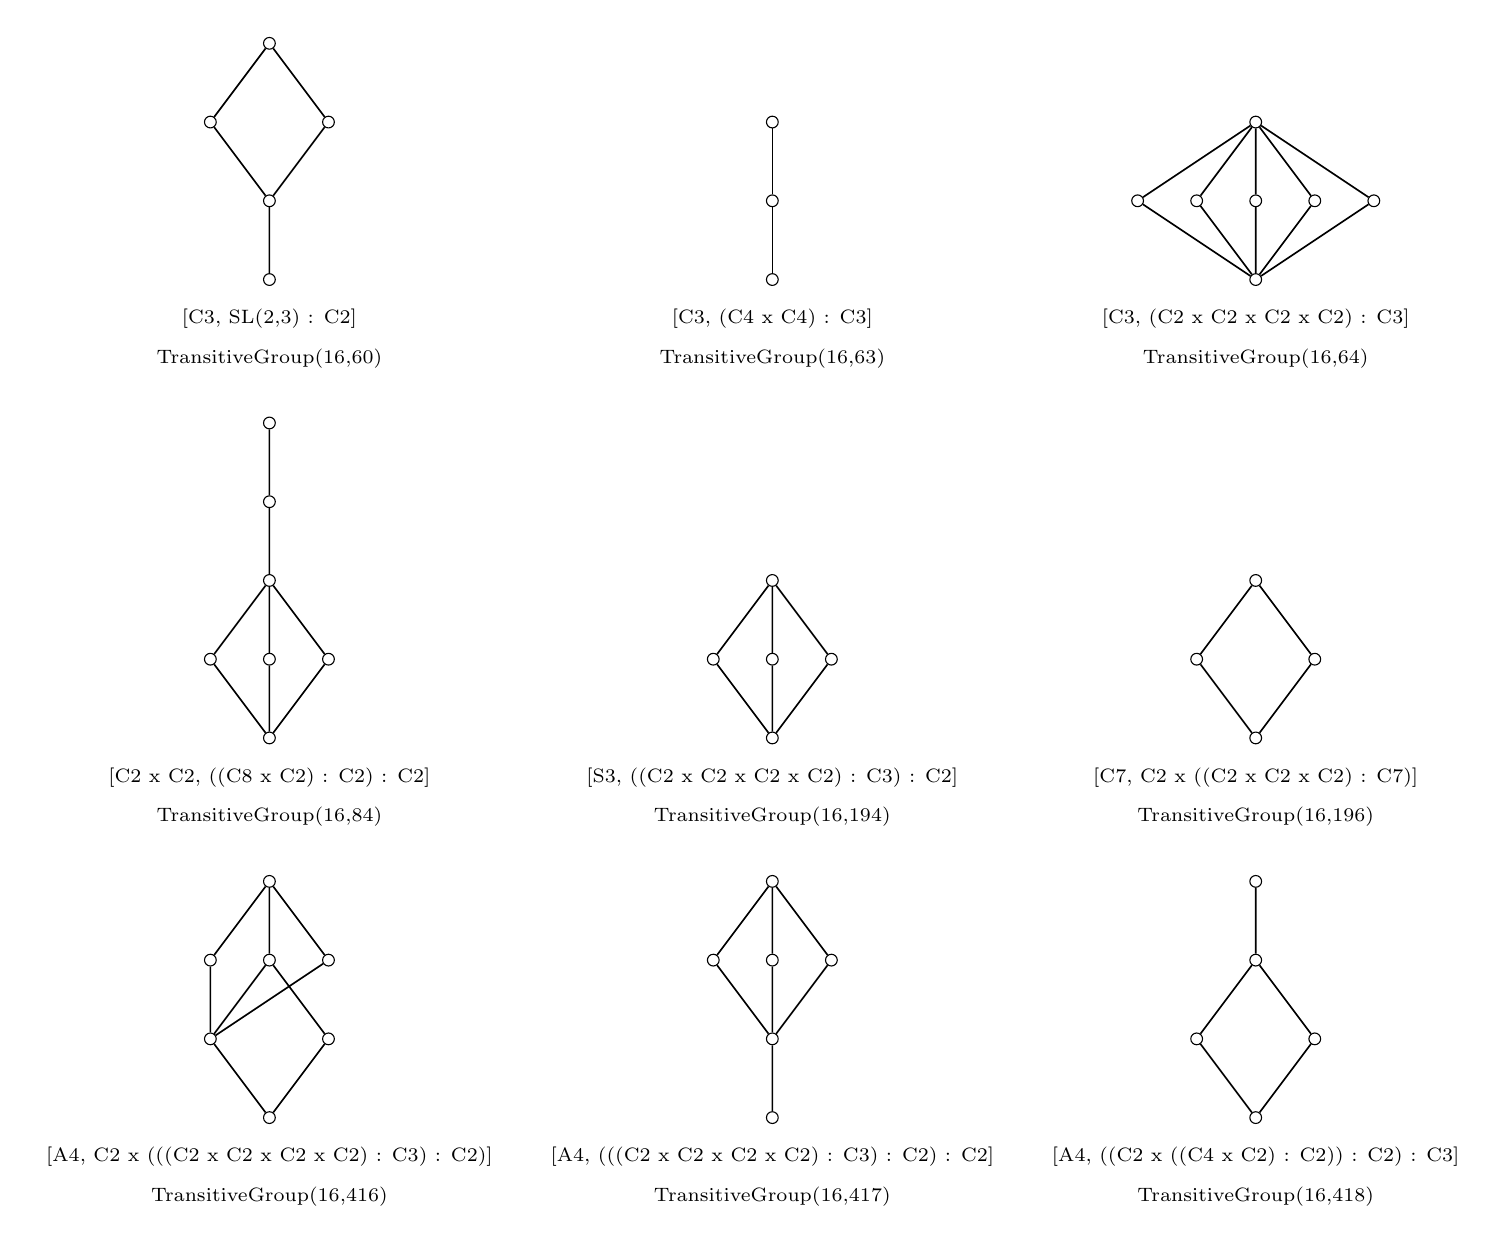
\begin{tikzpicture}[scale=.5]
\matrix[column sep=5mm,row sep=5mm]
{
\node (0) at (0,0) [draw, circle,inner sep=1.5pt] {};
\node (1) at (-0,1) [draw, circle, inner sep=1.5pt] {};
\node (2) at (0.75,2) [draw, circle, inner sep=1.5pt] {};
\node (3) at (-0.75,2) [draw, circle, inner sep=1.5pt] {};
\node (4) at (-0,3) [draw, circle, inner sep=1.5pt] {};
\draw[font=\scriptsize] (0,-.5) node {[C3, SL(2,3) : C2]};
\draw[font=\scriptsize] (0,-1) node {TransitiveGroup(16,60) };

\draw[semithick]
(0) to (1)
(1) to (2)
(1) to (3)
(2) to (4)
(3) to (4);
&
\node (0) at (0,0) [draw, circle,inner sep=1.5pt] {};
\node (1) at (-0,1) [draw, circle, inner sep=1.5pt] {};
\node (2) at (-0,2) [draw, circle, inner sep=1.5pt] {};
\draw[font=\scriptsize] (0,-.5) node {[C3, (C4 x C4) : C3]};
\draw[font=\scriptsize] (0,-1) node {TransitiveGroup(16,63) };

\draw[semithick]
(0) to (1)
(1) to (2);
&
\node (0) at (0,0) [draw, circle,inner sep=1.5pt] {};
\node (1) at (-0,1) [draw, circle, inner sep=1.5pt] {};
\node (2) at (0.75,1) [draw, circle, inner sep=1.5pt] {};
\node (3) at (-0.75,1) [draw, circle, inner sep=1.5pt] {};
\node (4) at (1.5,1) [draw, circle, inner sep=1.5pt] {};
\node (5) at (-1.5,1) [draw, circle, inner sep=1.5pt] {};
\node (6) at (-0,2) [draw, circle, inner sep=1.5pt] {};
\draw[font=\scriptsize] (0,-.5) node {[C3, (C2 x C2 x C2 x C2) : C3]};
\draw[font=\scriptsize] (0,-1) node {TransitiveGroup(16,64) };

\draw[semithick]
(0) to (1)
(0) to (2)
(0) to (3)
(0) to (4)
(0) to (5)
(1) to (6)
(2) to (6)
(3) to (6)
(4) to (6)
(5) to (6);
\\
\node (0) at (0,0) [draw, circle,inner sep=1.5pt] {};
\node (1) at (-0,1) [draw, circle, inner sep=1.5pt] {};
\node (2) at (0.75,1) [draw, circle, inner sep=1.5pt] {};
\node (3) at (-0.75,1) [draw, circle, inner sep=1.5pt] {};
\node (4) at (-0,2) [draw, circle, inner sep=1.5pt] {};
\node (5) at (-0,3) [draw, circle, inner sep=1.5pt] {};
\node (6) at (-0,4) [draw, circle, inner sep=1.5pt] {};
\draw[font=\scriptsize] (0,-.5) node {[C2 x C2, ((C8 x C2) : C2) : C2]};
\draw[font=\scriptsize] (0,-1) node {TransitiveGroup(16,84) };

\draw[semithick]
(0) to (1)
(0) to (2)
(0) to (3)
(1) to (4)
(2) to (4)
(3) to (4)
(4) to (5)
(5) to (6);
&
\node (0) at (0,0) [draw, circle,inner sep=1.5pt] {};
\node (1) at (-0,1) [draw, circle, inner sep=1.5pt] {};
\node (2) at (0.75,1) [draw, circle, inner sep=1.5pt] {};
\node (3) at (-0.75,1) [draw, circle, inner sep=1.5pt] {};
\node (4) at (-0,2) [draw, circle, inner sep=1.5pt] {};
\draw[font=\scriptsize] (0,-.5) node {[S3, ((C2 x C2 x C2 x C2) : C3) : C2]};
\draw[font=\scriptsize] (0,-1) node {TransitiveGroup(16,194) };

\draw[semithick]
(0) to (1)
(0) to (2)
(0) to (3)
(1) to (4)
(2) to (4)
(3) to (4);
&
\node (0) at (0,0) [draw, circle,inner sep=1.5pt] {};
\node (1) at (0.75,1) [draw, circle, inner sep=1.5pt] {};
\node (2) at (-0.75,1) [draw, circle, inner sep=1.5pt] {};
\node (3) at (-0,2) [draw, circle, inner sep=1.5pt] {};
\draw[font=\scriptsize] (0,-.5) node {[C7, C2 x ((C2 x C2 x C2) : C7)]};
\draw[font=\scriptsize] (0,-1) node {TransitiveGroup(16,196) };

\draw[semithick]
(0) to (1)
(0) to (2)
(1) to (3)
(2) to (3);
\\
\node (0) at (0,0) [draw, circle,inner sep=1.5pt] {};
\node (1) at (0.75,1) [draw, circle, inner sep=1.5pt] {};
\node (2) at (-0.75,1) [draw, circle, inner sep=1.5pt] {};
\node (3) at (-0,2) [draw, circle, inner sep=1.5pt] {};
\node (4) at (0.75,2) [draw, circle, inner sep=1.5pt] {};
\node (5) at (-0.75,2) [draw, circle, inner sep=1.5pt] {};
\node (6) at (-0,3) [draw, circle, inner sep=1.5pt] {};
\draw[font=\scriptsize] (0,-.5) node {[A4, C2 x (((C2 x C2 x C2 x C2) : C3) : C2)]};
\draw[font=\scriptsize] (0,-1) node {TransitiveGroup(16,416) };

\draw[semithick]
(0) to (1)
(0) to (2)
(1) to (3)
(2) to (3)
(2) to (4)
(2) to (5)
(3) to (6)
(4) to (6)
(5) to (6);
&
\node (0) at (0,0) [draw, circle,inner sep=1.5pt] {};
\node (1) at (-0,1) [draw, circle, inner sep=1.5pt] {};
\node (2) at (-0,2) [draw, circle, inner sep=1.5pt] {};
\node (3) at (0.75,2) [draw, circle, inner sep=1.5pt] {};
\node (4) at (-0.75,2) [draw, circle, inner sep=1.5pt] {};
\node (5) at (-0,3) [draw, circle, inner sep=1.5pt] {};
\draw[font=\scriptsize] (0,-.5) node {[A4, (((C2 x C2 x C2 x C2) : C3) : C2) : C2]};
\draw[font=\scriptsize] (0,-1) node {TransitiveGroup(16,417) };

\draw[semithick]
(0) to (1)
(1) to (2)
(1) to (3)
(1) to (4)
(2) to (5)
(3) to (5)
(4) to (5);
&
\node (0) at (0,0) [draw, circle,inner sep=1.5pt] {};
\node (1) at (0.75,1) [draw, circle, inner sep=1.5pt] {};
\node (2) at (-0.75,1) [draw, circle, inner sep=1.5pt] {};
\node (3) at (-0,2) [draw, circle, inner sep=1.5pt] {};
\node (4) at (-0,3) [draw, circle, inner sep=1.5pt] {};
\draw[font=\scriptsize] (0,-.5) node {[A4, ((C2 x ((C4 x C2) : C2)) : C2) : C3]};
\draw[font=\scriptsize] (0,-1) node {TransitiveGroup(16,418) };

\draw[semithick]
(0) to (1)
(0) to (2)
(1) to (3)
(2) to (3)
(3) to (4);
\\
};
\end{tikzpicture}
\end{center}
\end{figure}

\newpage

\begin{figure}[h]
\caption{Transitive G-set congruence lattices in Eq(16) (continued)}
\label{fig:16c}
\begin{center}
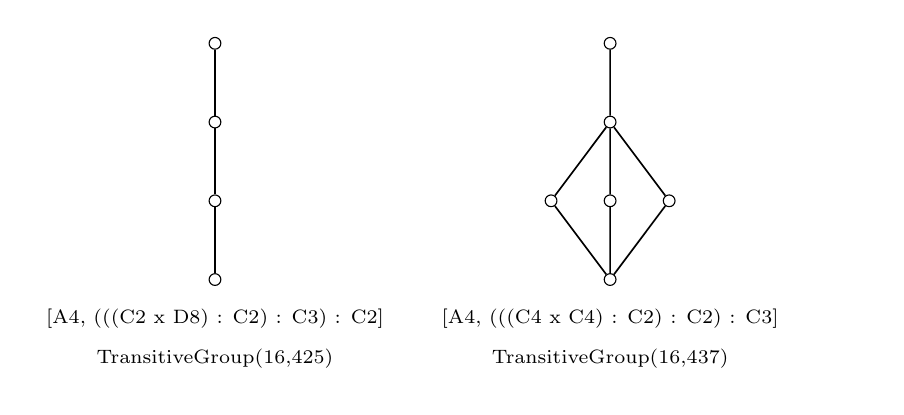
\begin{tikzpicture}[scale=.5]
\matrix[column sep=5mm,row sep=5mm]
{
\node (0) at (0,0) [draw, circle,inner sep=1.5pt] {};
\node (1) at (-0,1) [draw, circle, inner sep=1.5pt] {};
\node (2) at (-0,2) [draw, circle, inner sep=1.5pt] {};
\node (3) at (-0,3) [draw, circle, inner sep=1.5pt] {};
\draw[font=\scriptsize] (0,-.5) node {[A4, (((C2 x D8) : C2) : C3) : C2]};
\draw[font=\scriptsize] (0,-1) node {TransitiveGroup(16,425) };

\draw[semithick]
(0) to (1)
(1) to (2)
(2) to (3);
&
\node (0) at (0,0) [draw, circle,inner sep=1.5pt] {};
\node (1) at (-0,1) [draw, circle, inner sep=1.5pt] {};
\node (2) at (0.75,1) [draw, circle, inner sep=1.5pt] {};
\node (3) at (-0.75,1) [draw, circle, inner sep=1.5pt] {};
\node (4) at (-0,2) [draw, circle, inner sep=1.5pt] {};
\node (5) at (-0,3) [draw, circle, inner sep=1.5pt] {};
\draw[font=\scriptsize] (0,-.5) node {[A4, (((C4 x C4) : C2) : C2) : C3]};
\draw[font=\scriptsize] (0,-1) node {TransitiveGroup(16,437) };

\draw[semithick]
(0) to (1)
(0) to (2)
(0) to (3)
(1) to (4)
(2) to (4)
(3) to (4)
(4) to (5);
&
& \\
};
\end{tikzpicture}
\end{center}
\end{figure}

\newpage


%\input{TransitiveGsetCongEx16CorefreeMin3Max14.tex}




%%%%%%%%%%%%%%%%%%%%   End of main body of article
%
%                             References
%
%   BiBTeX users uncomment the following line:
%
\bibliographystyle{plainurl} %jloganal}
%
\bibliography{refs}

%%%%%%%%%%% TOTO: Insert bibtex data here!! %%%%%%%%%%%%%%%%%%5

\end{document}


